% $Id: AllegProposal.tex,v 1.8 2000/07/05 21:02:12 culver Exp $
% AllegProposal.tex
% by A. Thall
% 13. Feb 2003
%
% Small edits and a few additions made by R. Roos
% 21 Jan 2007
% Most particularly, the "box" around the thesis statement has been removed,
% section titles have been modified. The section named "Prior work II" has
% been commented out. The \topmargin has been changed to -.5in and the
% change to \parindent has been commented out.
% The filename "nausicaa.eps" has been changed to simply "nausicaa" so that
% pdflatex can be used on the file (and a file named "nausicaa.pdf" has
% been created using the "epstopdf" command).
% Several subsections have been added to illustrate subsection usage.
% The word "comp" has been replaced by "project" or "thesis" throughout.
% Other small changes have been made.
%
% This document provides a sample Senior Project Proposal template for use
% by students in Allegheny's CS and Applied Computing programs.

\NeedsTeXFormat{LaTeX2e}
\documentclass[11pt]{article}

%The following is used by WinEdt to set up cross-referencing to the BibTeX files
%It is NOT commented out---the comment lets it be simply ignored by non-WinEdt LaTeX compilers

%GATHER{mybibtexDB.bib}

\usepackage{setspace}
\usepackage{amsmath}
\usepackage{amssymb}
\usepackage{epsfig}
\usepackage{fancybox}
\usepackage{listings}
\usepackage{algo}
\usepackage{url}

%----------My added Packages-----------------
\usepackage{soul}
\usepackage{graphicx}
\usepackage{amsthm}
\newtheorem{ProposalDef}{Definition}
\usepackage{color}
\newcommand{\hilight}[1]{\colorbox{yellow}{#1}}

\usepackage{titlesec}
\titleformat{\subsubsection}[runin]{\normalfont\bfseries}{}{}{}[]

\soulregister{\em}{1}
%-------------------------------------------------------

\setlength{\textheight}{9in}
\setlength{\textwidth}{6in}
\setlength{\oddsidemargin}{.25in}
\setlength{\topmargin}{-.5in}  % changed from -.25 by RSR on 1/21/07
%\parindent .5in    % commented out by RSR 1/21/07

%put words in the hyphenation statement if you want to enforce
%how LaTeX should break them (or not) at the end of a line.
%\hyphenation{repre-sen-tations problems exact linear}
\hyphenation{itself}

%%%%%
%% Commented out -- RSR, 1/21/07
%%%%%
% The following provides a box to surround the thesis statement
%\newenvironment{Thesis}%
%{\begin{Sbox}\begin{minipage}{.95\linewidth}}%
%{\end{minipage}\end{Sbox}\begin{center}\fbox{\TheSbox}\end{center}}

\title{Incremental Model Synchronization in Model Driven Engineering}
\author{Hamid Gholizadeh \\ Supervisor:  Dr. Tom Maibaum \\ 
Committee Members: Dr. Wolfram Kahl, Dr. Jacques Carette }

\begin{document}

% You can specify a language and other options for
% the code-formatting "listings" package
\lstset{language=C++,basicstyle=\small,
        stringstyle=\ttfamily,showstringspaces=false}

\singlespace
\maketitle

\begin{abstract}                % ~350 words max
Model Driven Engineering (MDE) is proven to be a promising approach in software engineering. software model consistency management and maintenance stands at the core of the MDE procedure while it still needs more theoretical and technical supports for realization of its required functionalities like model transformation, synchronization and change propagation. 
In this thesis proposal we explore the type of different synchronization scenarios in Model Driven Software Engineering, and will introduce three areas which needs more contribution and research : private/shared parts, least/minimal change application, and concurrent synchronization and conflict resolution. 
\end{abstract}

\doublespace
% This sets section-numbering to only include Section and Subsection numbers
\setcounter{secnumdepth}{2}

\section{Introduction}\label{ch:overview}

MDE (Model Driven Engineering) is proven to be a demanding approach in software development process \cite{Brambilla:MDE:2012dq,Bezivin:MDA:2004nx}. One of the intentions of the MDE approach in Software Development is to bring the intelligence of the human being to the more abstract level of models rather than concrete level of the codes. In Model Driven Software Engineering (MSDE), models are to be considered as active and first-class citizens of the software engineering process artifacts as opposed to the current practice where models --like UML diagrams-- are usually used as a supportive and rather passive artifacts, e.g. for software development team inter-communications. The latter happened because of lack of complete formality and tool support for maintaining models; for example {\em Model Management} as a core task of MDE, still lacks enough formal foundation and applicable tools, supporting its demanded functionalities like {\em Model Correspondence Specification} and its maintenance in terms of {\em Model Synchronization} or {\em Change Propagation},  and {\em Conflict resolution.} 
There are still many research at the moment on some other aspects of {\em Model Management} like {\em Model Transformation} which is discussed in the Section \ref{sec:Lit} in more details.

In a typical practice of software engineering process, models are evolving  form more abstract levels to more concrete level-- from Specification to implementation by code. We call this process {\em model refinement} and can look at it like vertical movement from more abstract levels to less abstract ones. This {\em Vertical}  --up to down-- movement usually happens in reverse direction too where it is called {\em reverse engineering}-- to fit in and accomplish the iterative method of software development process. This up and down process, then is called {\em round-trip engineering}. During round-tripping process, sometimes it is necessary to move between the models at the same levels of abstraction --movement not changing the level of abstraction, Therefore it is called horizontal movement as apposed the latter vertical movement. However, ike the previous case this movement can be in forward and backward directions (Figure  \ref{fig:model-code}.)

%:Key private-shared Picture
 \begin{figure}[ht!]
\centering
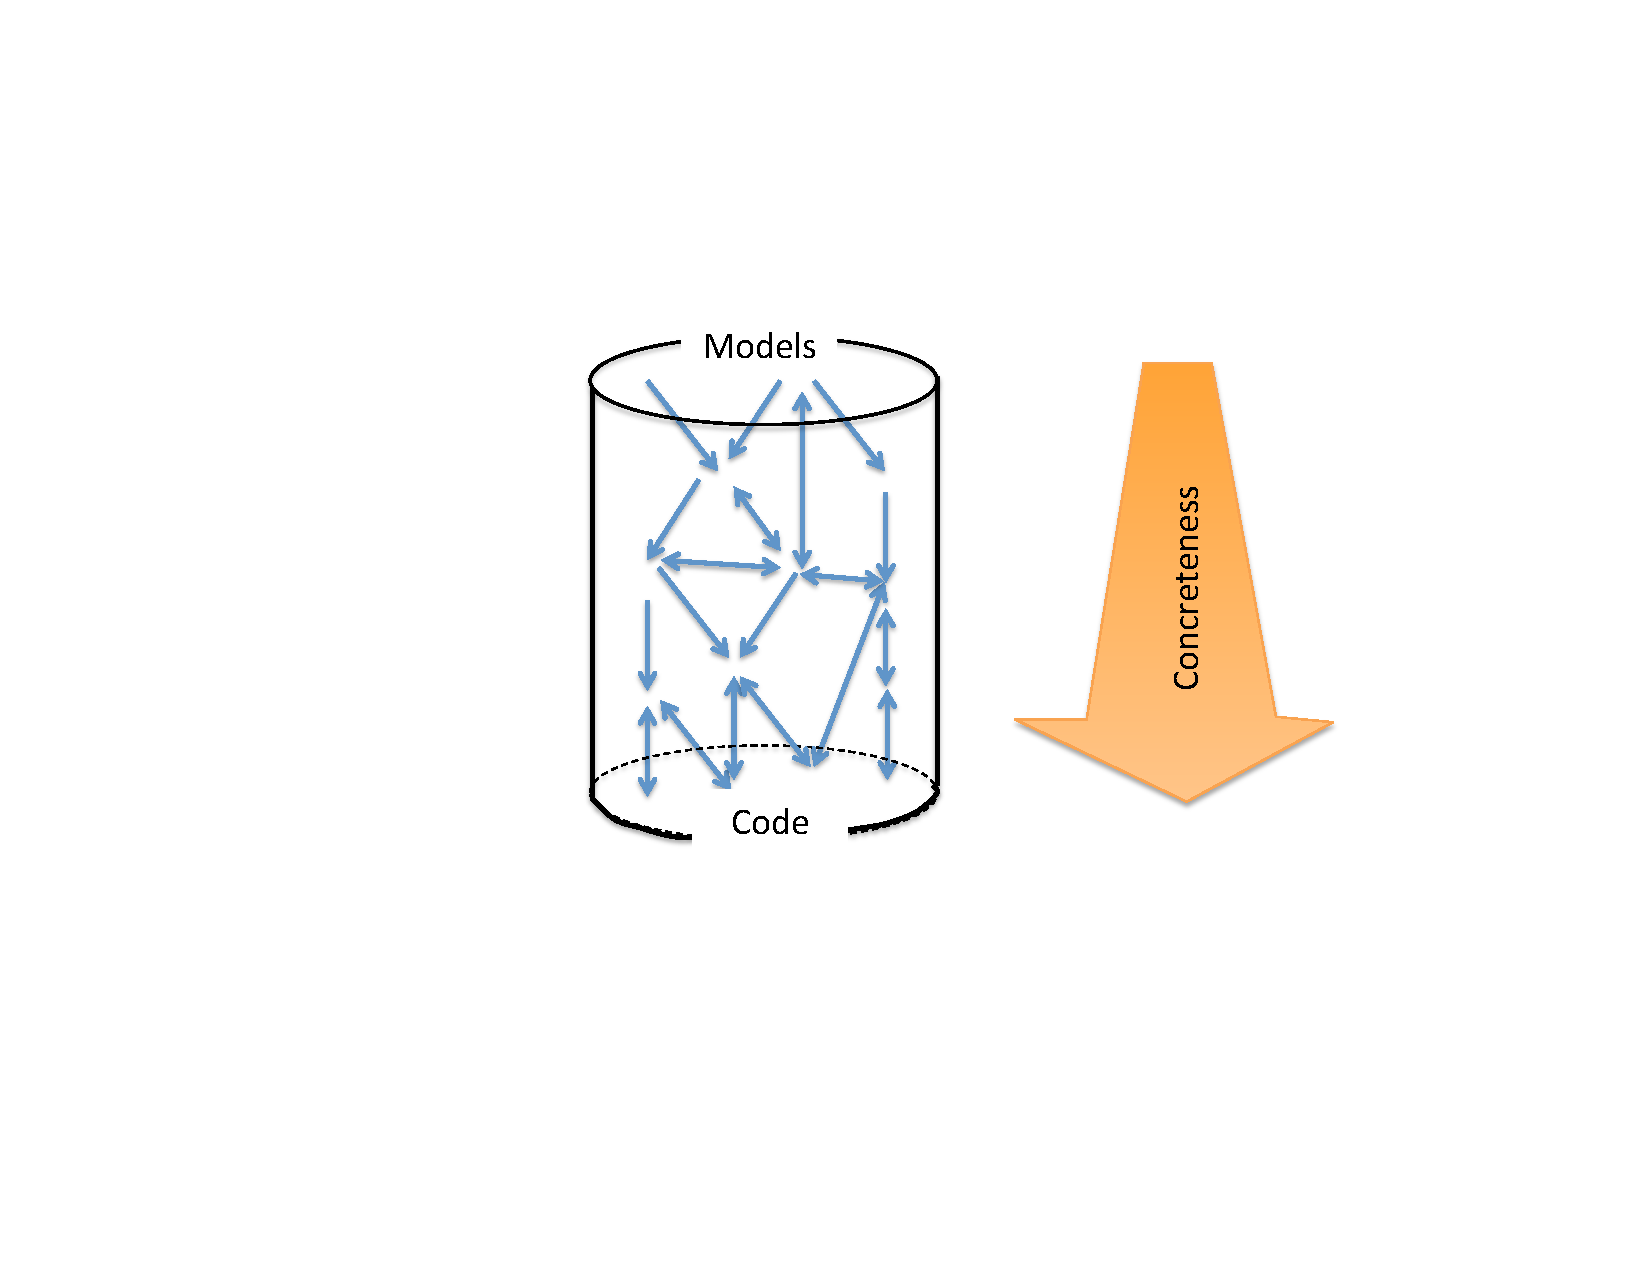
\includegraphics[width=50mm]{images/model-code}
\caption{Vertical and Horizontal movements in software eng.}
\label{fig:model-code}
\end{figure}


The horizontal movement is necessary because each model might demonstrate and focus on different aspects of the software system, or maybe some models are suitable for different users to work with. For example, in a typical development process of software development using UML diagrams \footnote{we consider diagrams as models, but not the other way around, i.e. models not need to be diagrammatic.}, each model share some common parts with other models and some have their own specific features. E.g. {\em Class Diagram} and {\em State Chart} diagram can share some of the class method signatures, while attribute names for the classes, and the order of the events happening, are correspondingly considered as specific and private parts of each.

Because of the inevitable changes which is frequently happing during the software development process, and also during the maintenance phase \cite{Briand:UMLChangeMng:2013cr}, it is necessary to handle the {\em change propagation} which is actually is the semantic of the ``movement'' in previous paragraph. Hence change propagation can happen {\em Vertically} or {\em Horizontally}. 
%By {\em Vertical} change propagation we mean a Model {\em refinement} from more abstract level to more concrete one or vice versa. By {\em Horizontal} refinement we mean change propagation among the models, since they are sharing some concept together as discussed in previous paragraph. 
Taking software artifacts a models, industrial projects would include hundreds or even thousands of models which are inter-related to each other in some ways, so changing one of them would require change propagation throughout the whole system. Handling this situation by hand without a tool support, even in small scale scenarios is tedious, complicated, error-prone and very time-consuming and for the large cases, is nearly impossible. That is why nowadays, most changes are applied directly on codes rather than models, which made software engineering deprived of many proved benefit of Model Driven Software Development. That is ending up with inconsistent artifacts of the software development which is the typical story of the large scale software projects, then most of them are usually looked as outdated historical records and decorative pieces rather than the live, influential  and dependable software artifacts.
%{\em Software artifacts other than code is so important that \cite{Fundamental of Information Technology} defines software as a programming code plus the modelling artifacts and documentations.} 

Change propagation among the models are also called {\em model synchronization}, in the sense that it makes the involved models consistent and synchronized after changes on one model is propagated to the others. In following section we will discuss by example different aspects of the model synchronization and will identify 3D orthogonal dimensions of the synchronization scenarios. We also would examine the bidirectional model synchronization and synchronizer transformers properties and will introduce the formal representation of the models.  Following those, we will identify three connected problems in domain of model synchronization in section \ref{sec:Problem} which is the subject of this thesis proposal. We will discuss related works in section \ref{sec:Lit} and will propose the approach to the problem solution and conclude in section \ref{sec:conclusion}.

%\footnote{More details and formalization of these dimensions is submitted to the MODELS 2013 conference in Miami, Florida - USA}

%This thesis proposal examines underlying formalities and existing works in the area of  {\em Model Synchronization} and identifying some gaps in current works and motivates how addressing those gaps is necessary in specification and implementation of formal synchronization framework, since it  would provide formal foundation for verifying the implemented synchronization framework. To be more specific we intend to address the formalities underlining the {\em Shared} and {\em Private} parts of the related models which matters in {\em Model Synchronization}. More detailed discussion on the problem is covered in section \ref{sec:Problem}. We will also discuss briefly some other  open problems, including {\em Concurrent Model Synchronization} and {\em Conflict Resolution} strategies $-$ which might  be an extended work of this research, that we observed during the survey on {\em Model Synchronization} area for future reference.





\section {Context of the Synchronization Scenarios}\label{subsec:SynchScen}
%\section{3-Dimension of Synchronization Scenarios} 
In this section we describe the three dimensions of the synchronization scenarios: {\em Organizational Symmetry}, {\em Information Symmetry} and {\em Incrementality}, which are orthogonal(independent) to each other, in the sense that each is describing an independent aspect of the synchronization scenario. For describing these concepts we will start with an example from a flight reservation system which is modeling a simple flight arrangement and implementation in a typical airline company. later we will introduce the 3D dimension and discuss them in more details. Formal definition of each dimension is presented in our recent work submitted to MODELS13 conference \cite{Zinovy:2013:OCC:Symmet}. We will also discuss the concurrency dimension and its relation to later synchronization dimensions. Later we will discuss the concept of Bidirectional Transformation and will introduce properties of the synchronizer transformers. At the end of this section we will introduce typed attributed graphs which is introduced as a formal foundation of the model and meta-modeling concepts.

\subsection{Flight Databse Example}
\label{sub:example}
Suppose that there are two groups of employee in an airline company. One group is responsible for identifying the business aspect of the flights and identify the necessary flights which should be set between different destinations according to the airline business and marketing policies. Another group in more technical and trying to implement defined flights by group one (Figure \ref{fig:Example01}). For example flight \#11 in Model A is implemented by two flights \#1 and \#2 in Model B. For specifying the relation (implementation) of Model A with Model B, we define an intermediate view over Model B --get(B), which is actually an implementation of the Model A. Intermediate View is pair of (self.fst, self,scd) where :

(Q)  \textsf{self.fst.to $=$ self.snd.from} \mbox{ and } \textsf{self.fst.time $\le$ self.snd.time}.

 \begin{figure}[ht!]
\centering
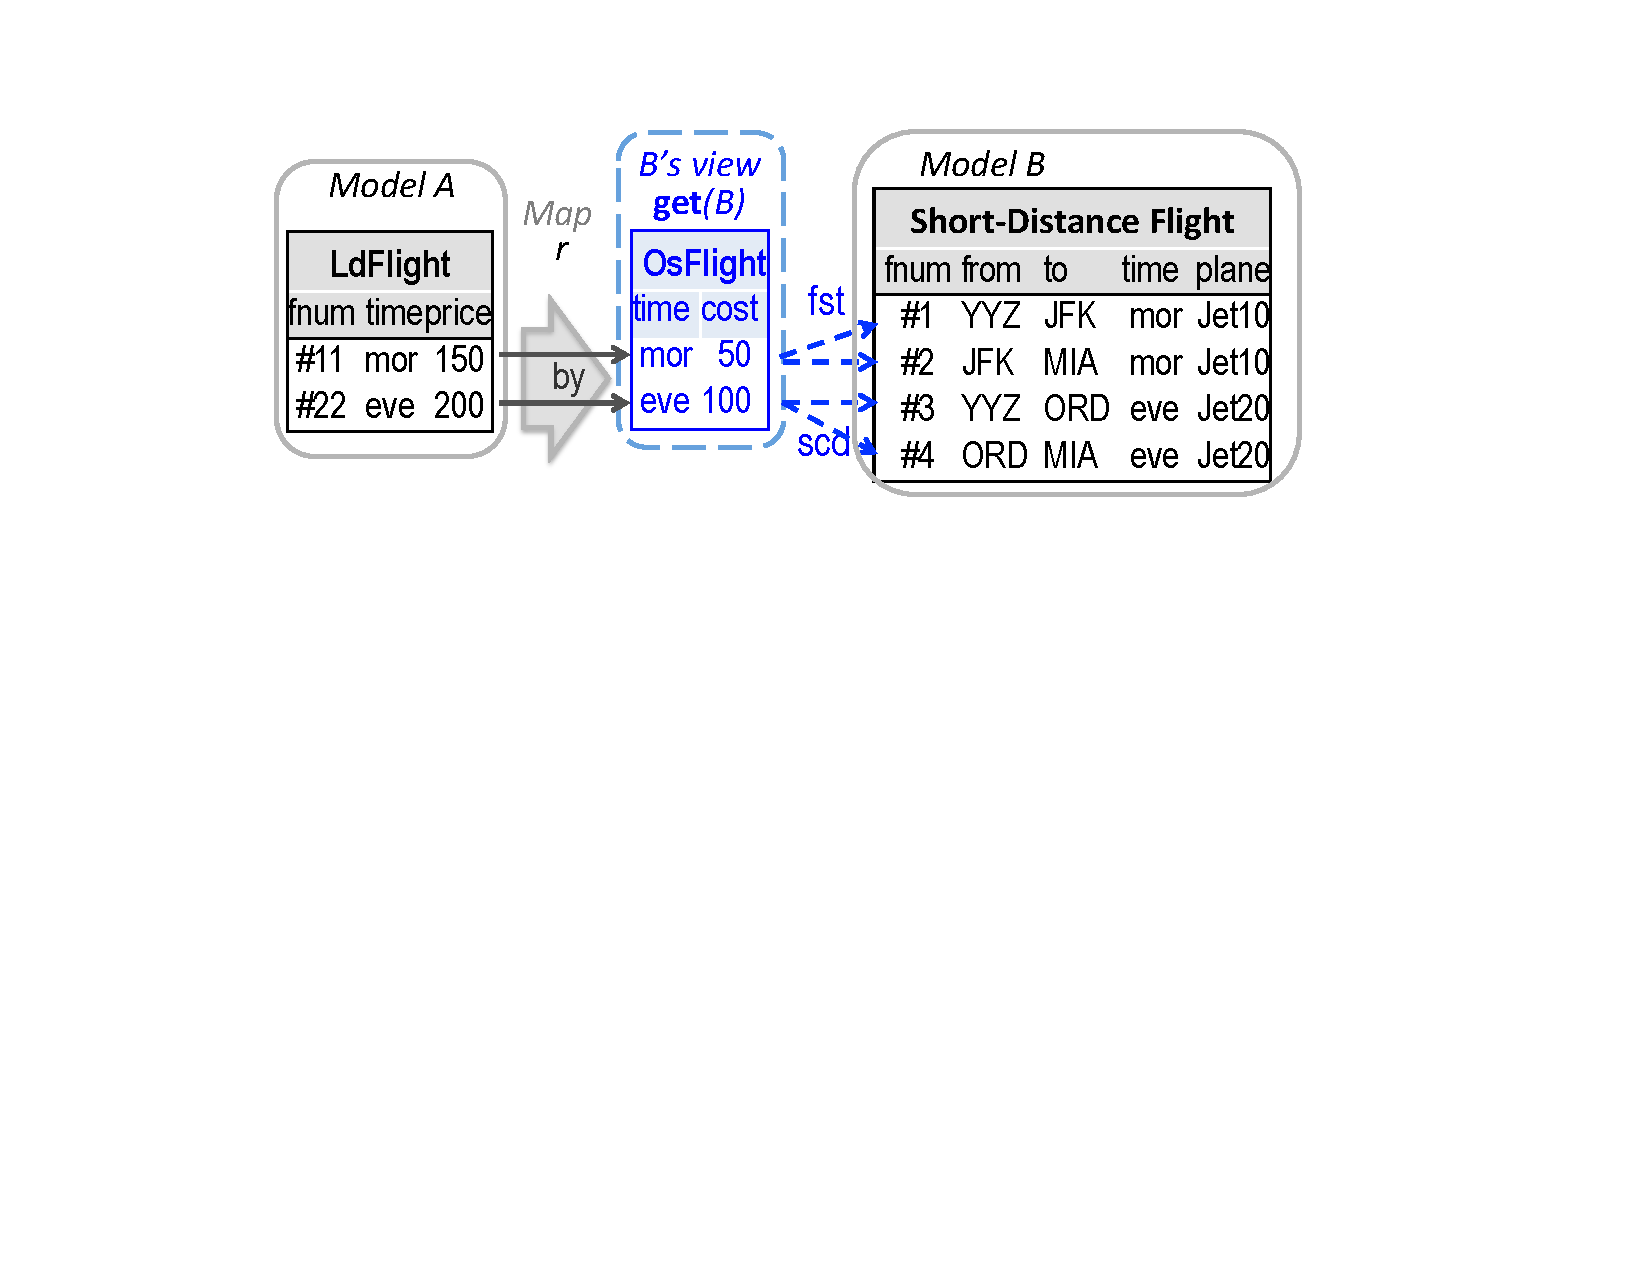
\includegraphics[width=100mm]{images/Example01}
\caption{Model B and mapping r implement model A}
\label{fig:Example01}
\end{figure}

 \noindent We also define \textsf{self.time=self.fst.time}. Computing \textsf{self.cost} is done by some procedure using airport and airplane data.  So we can have a function \verb+get(B)+ that computes derived table OsFlight from base table SdFlight. Two 'by'-links relate Ld-flights to their one-stop implementations. Together they form an inter-table (sub)mapping \textsf{by: LdFlight $\rightarrow$ OsFlight}, which constitutes a {\em model-correspondence mapping}  
 \textsf{$r:A \rightarrow get(B)$} (mapping $r$ could contain more submappings like \textsf{by}, if model $A$ would have more tables/classes). Note that implementation is a pair $(B, r)$, but we will often say `implementation' $B$, leaving the correspondence mapping implicit.  We consider implementation $(B, r) $ to be \emph{correct}, if for each ld-flight \textsf{self} we have: %there is an os-flight  such that

   \noindent (C) $\mathsf{self.time=self.by.time} \mbox{ and } \mathsf{self.price} \ge \mathsf{self.by.cost} + 100 . %\leqno (C)
   \label{page:consistency}$

 \begin{figure}[ht!]
\centering
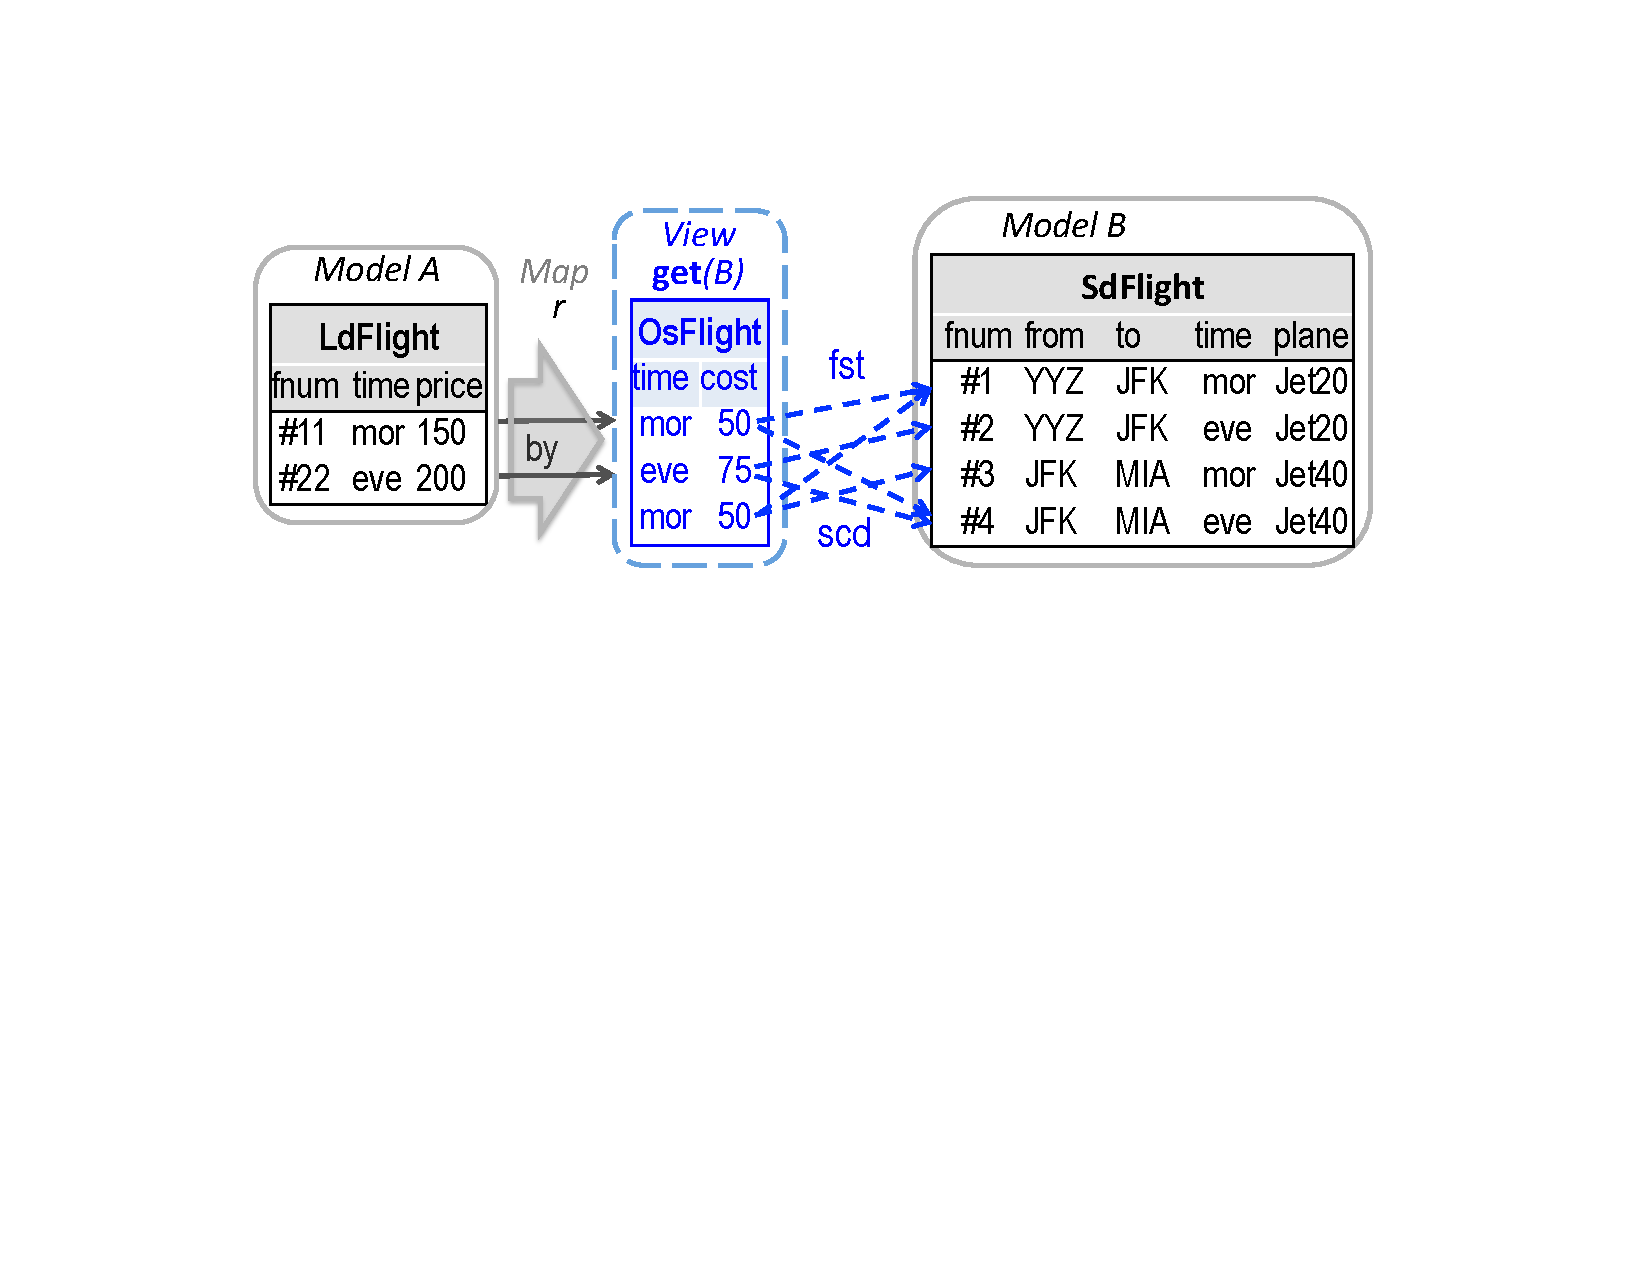
\includegraphics[width=100mm]{images/Example02}
\caption{Another Implementation for model A}
\label{fig:Example02}
\end{figure}


According to above definition, it is possible to have many implementation (B,r) for the same A. For example Figure \ref{fig:Example02} shows another implementation for the same LdFlight. This is the typical situation for the implementation of the models in software development where many alternative implementation is possible for the same model. It somehow indicates that there are some {\em Private} parts in the model B which is hidden from Model A's perspective, e.g. the \textsf{plane} and intermediate stops. From another side, the \textsf{fnum} information of the Model A is not reflected in \verb+get(B)+ view. This is the typical case of {\em Information Symmetric} scenario in model synchronization where each models have their own non-empty {\em private} parts. 

 \begin{figure}[ht!]
\centering
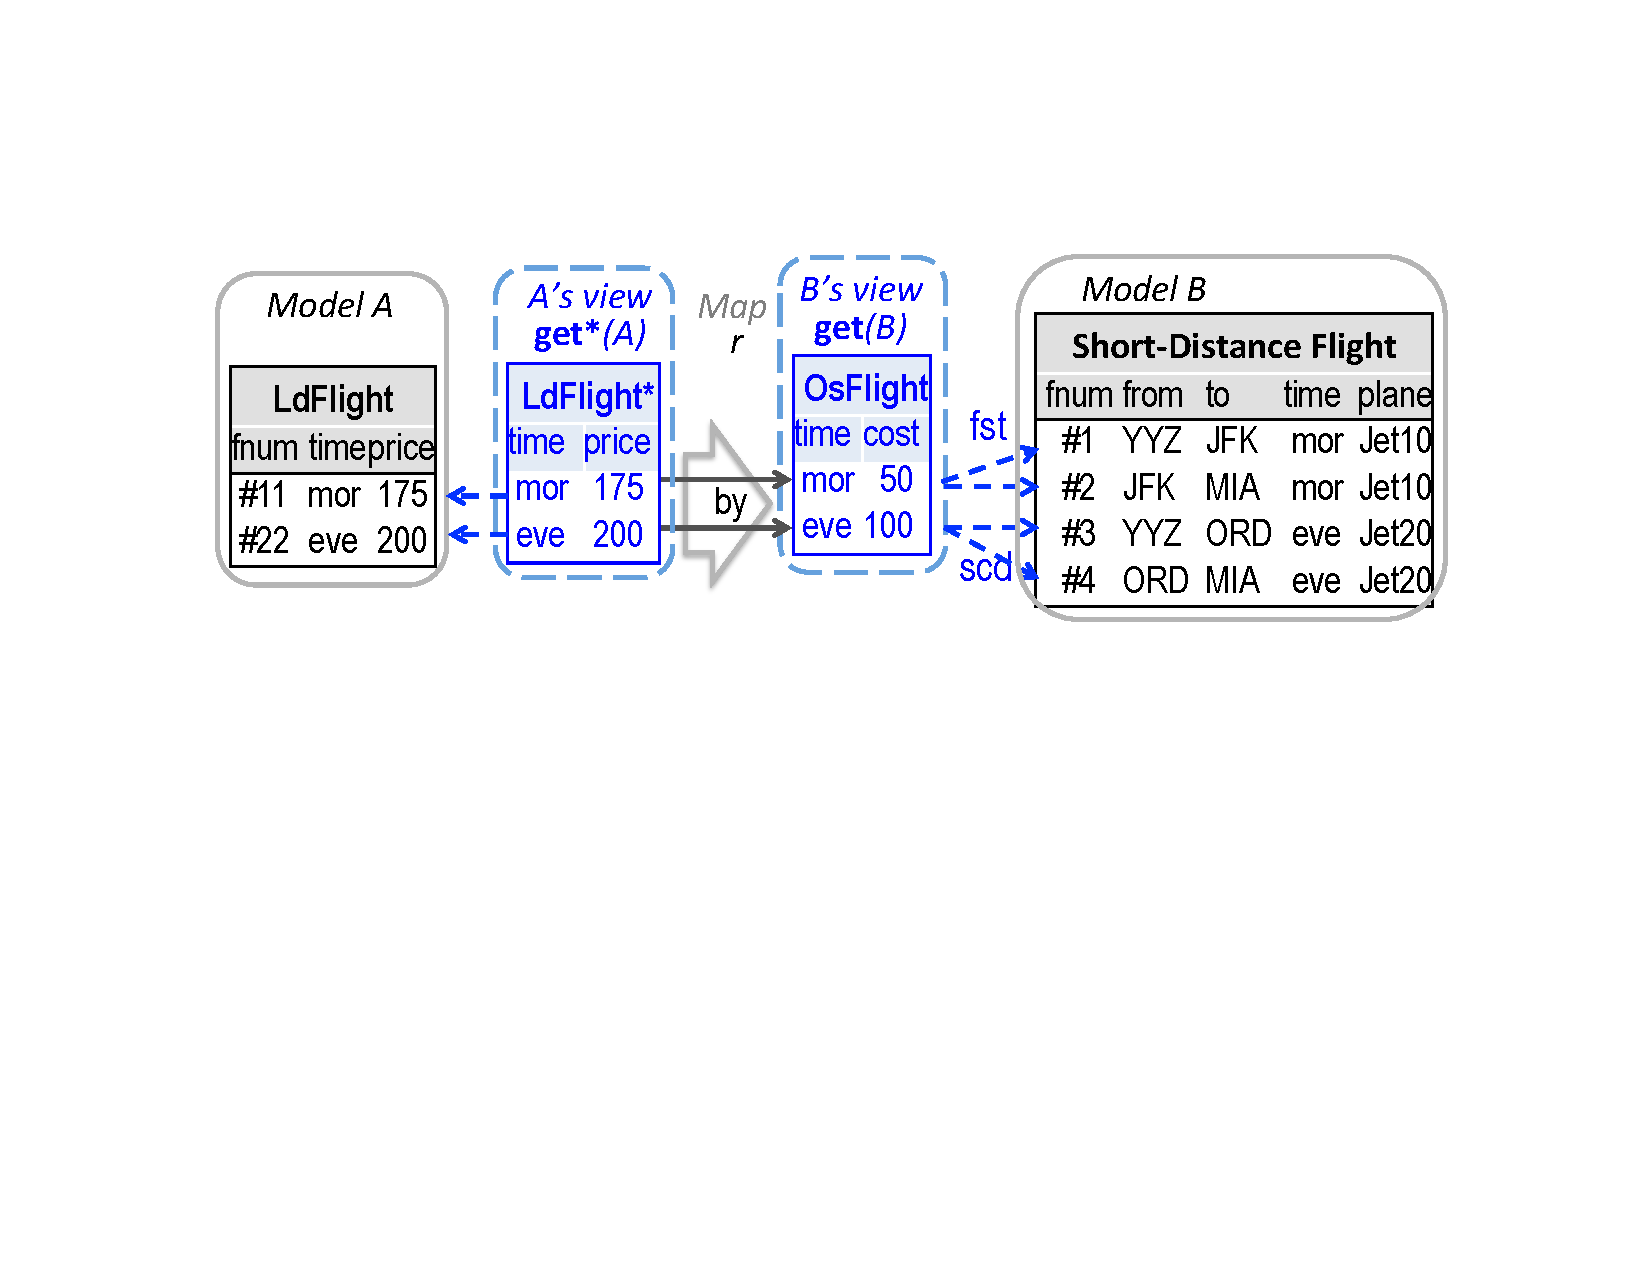
\includegraphics[width=100mm]{images/Example03}
\caption{Model B and mapping r implement model get*(A)}
\label{fig:Example03}
\end{figure}


If we make Figure \ref{fig:Example02} more elaborate,  we can indicate the mapping ``by'', from a projection of A (\verb+get+$^*$\verb+(A)+) to \verb+get(B)+ like Figure \ref{fig:Example03}. The project \verb+get+$^*$\verb+(A)+ would be a view on Model A where all its  information is completely dependent on Model A. In another word there is not private information in \verb+get+$^*$\verb+(A)+ which can not be obtained from Model A. This is the typical situation of the {\em Informationally Asymmetric} cases. Taking example above as the basis we continue to discuss different possible scenarios on that, exemplifying some of synchronization types which we will discuss classifying in 3D space later on. 


\subsubsection{Implementation is derived from the marketing decisions}, and the user doesn't care how the flights are implemented by the technical team. Model A has dominacy over Model B in the sense that either there is no independent work on Model B and it is just created using Model A, or if for users working on Model B, it is not important if their changes are discarded. This doesn't seem a good idea in the context of our example, but it might happen in the case of code generation. we will refer to this case as {\em Organizationally Asymmetric} case and we say that Model A {\em Organizationally} dominates Model B.


\subsubsection{Implementation needs to be preserved,} and discarding all changes on implementation when a change is happening on model A is disappointing. This is the most desirable cases in the common cases of the synchronization scenarios. A solution is to implement changes on side $A$ incrementally as shown in Figure \ref{fig:Example04}:  the change, or \emph{delta}, on side $A$, $\Delta_A$, is propagated to a delta on side $B$, $\Delta_B$, which together with the original implementation $B$ provides an updated implementation. In the figure, solid lines and shaded tables refer to given data, and dashed lines and blank tables denote data produced by the operation of delta propagation. In more detail, $\Delta_A$ makes explicit that flight \#11 is preserved while flight \#22 is added. Correspondingly, delta $\Delta_B$ keeps flights \#1 and \#2, and adds two Sd-flights implementing the required one-stop flight. The range of possible implementations is captured by placing \emph{labeled nulls}  $?_{i}$ into the table: nulls with the same labels must be substituted with the same values and nulls with different labels are independent, but may be also substituted with the same values. In this way, uncertain model $B'$ captures the implementations  in Figure \ref{fig:Example01}, and that one  in \ref{fig:Example02}, and many others possibilities. Correspondingly, the derived OsFlight table is also uncertain: the cost value is given by applying some known procedure say,  $F$, to unknown argument values  $?_{i}, i=1,2,3$. We term this kind of change propagation {\em Incremental Synchronization}.

\begin{figure}[ht!]
\centering
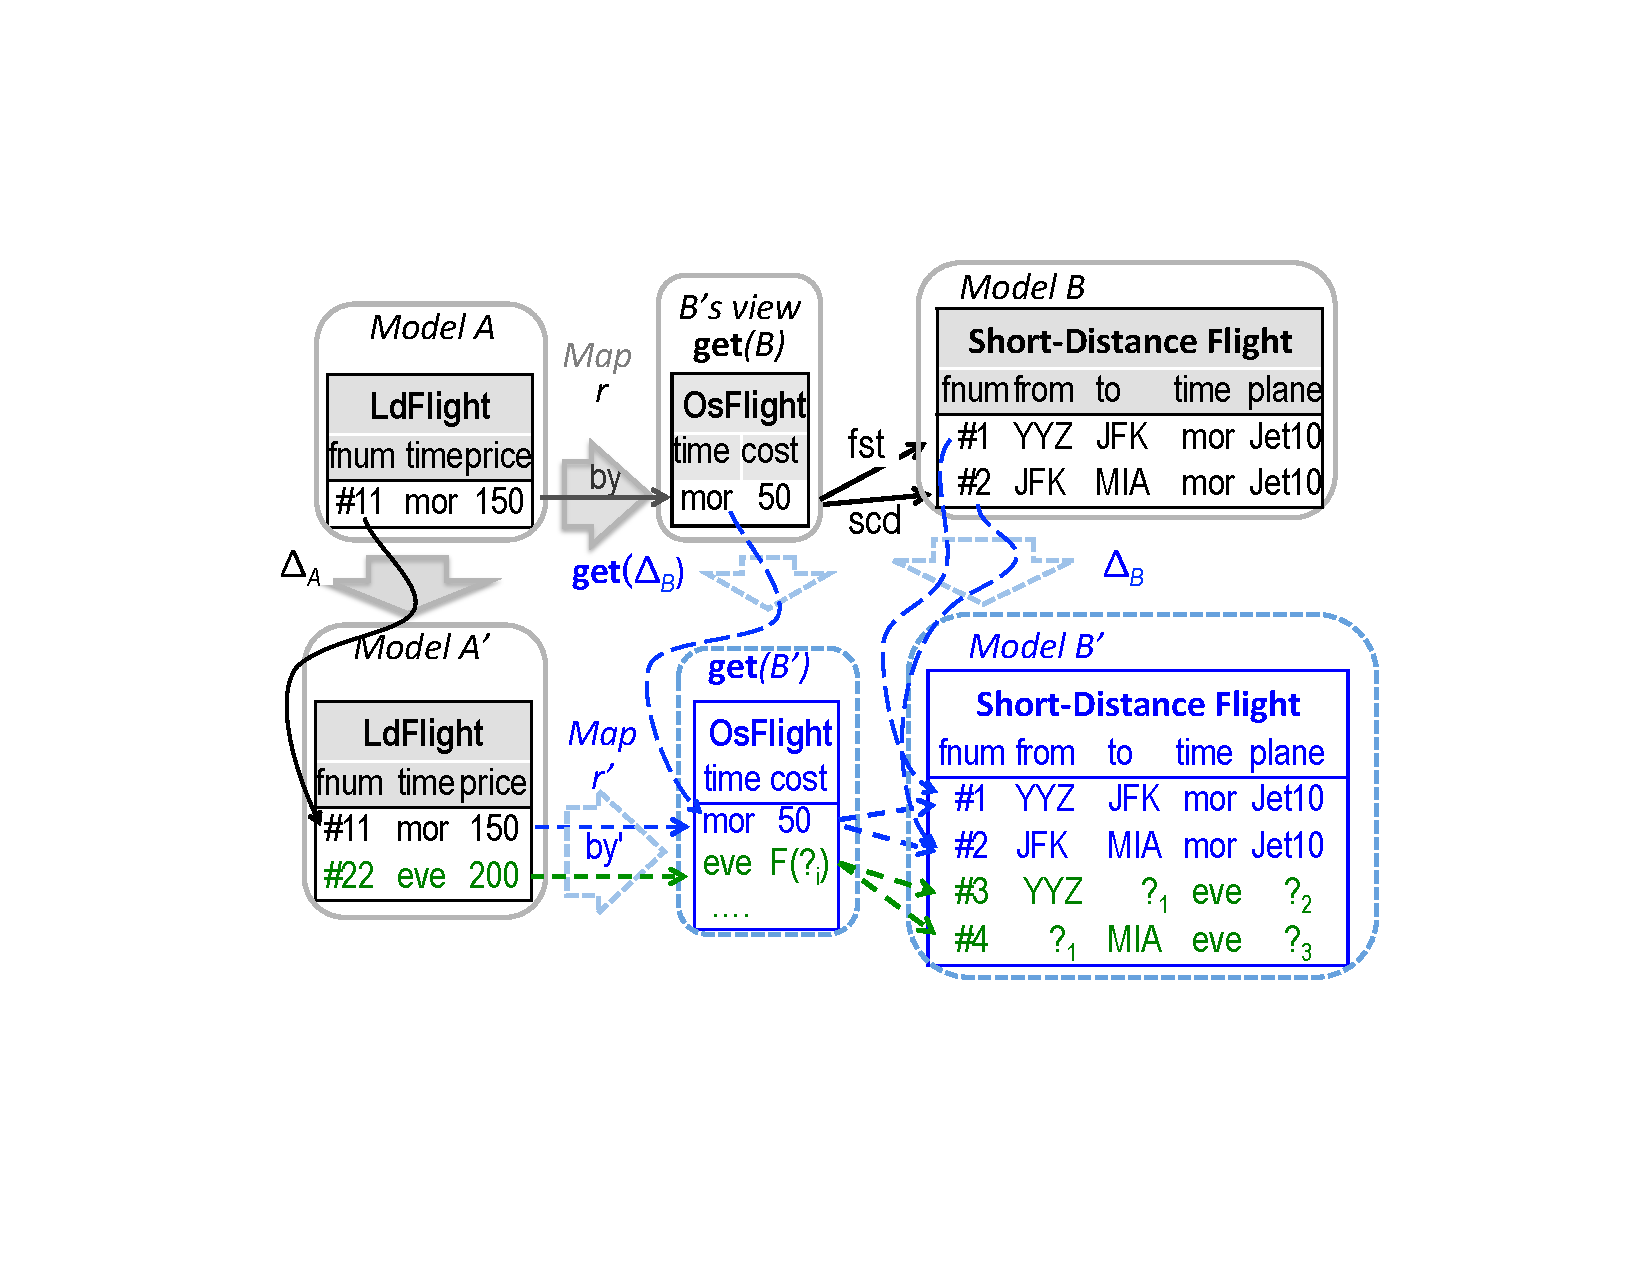
\includegraphics[width=100mm]{images/Example04}
\caption{Incremental implementation}
\label{fig:Example04}
\end{figure}

suppose that our policy impose that Model B can change to Model $B'$ as far as A and $B'$ are still consistent. Otherwise we will role back the changes to B. If so model B changes to consistent $B'$, in this case its changes would be respected while propagating changes from A to B. Though Model B would have more flexibility than the previous case where all changes are disregarded in update propagation from A to B. The latter policy also implies that we don't have a change propagation from B to A, so this situation is still {\em Organizational Asymmetry} but with {\em Incremental} updates.

%The extended version of these dimensions are discussed in our recent submitted paper in \cite{ICMT Paper with Zinovy}.


\subsubsection{Round-tripping or Organizational Symmetry.}

Consider a different business context, in which the technical team gains a greater authority and administrative weight than before. Now, if the technical team, while working with Model B originated from model $A$, would find a valuable modification  $B'$, e.g., new profitable os-flights, but $B'$ would be inconsistent with $A$, then the $B$-team may require to modify model $A$ to a state $A'$ consistent with $B'$.  In other words, unlike two previous cases, updates now can be propagated in both directions. We will refer to the case as \emph{Organizational Symmetry.}

\subsubsection {Organizational Semi-Symmetry or Partial Symmetry.}
Suppose the previous case of Round-tripping where update propagation allowed in both direction, and we deleted some information from Model A, for example, ld-flight \#11 in Figure \ref{fig:Example04} is deleted.  This deletion can be caused by a real world deletion of  sd-flight \textsf{\#11.fst: YYZ--JFK}, or\textsf{ \#11.scd: JFK--MIA}, or both.  We cannot arbitrarily choose one of them,  because objects of class SdFlight must represent actual flights existing in the schedule.  Hence, propagation of deletions in the Model $A$ must be prohibited. But as Figure \ref{fig:Example04} shows it is possible to propagate new addition from Model A to Model B. In another word some updates on Model A are allowed to be propagated to Model B but some are not. Note that this is more symmetric than the {\em Organizational Asymmetric} case and less symmetric than the {\em Organizational Symmetric} case. We call this case {\em Organizational Semi-Symmetric} case. %As we will discuss later this is independent of being {\em Informationally Symmetric} or {\em Asymmetric}

%\subsubsection {\hl {You might wan to discuss concurrency here}}

\subsection{Type Space of Synchronization Scenarios}
\label{sub:synchSpace}
Following from the previous section we identify 3 dimension of a synchronization types: (1){\em Organizational Symmetry}, (2){\em Informational Symmetry}, and (3){\em Incrementality}, ref. Figure \ref{fig:SynchTypePic}. We are going to briefly discuss each dimension; more details and their formalization can be found in submitted paper to MODELS13 conference \cite{Zinovy:2013:OCC:Symmet}.

%\hl{ need to match the examples on the 3D space}



%:Key Synchronization Types Picture
 \begin{figure}[ht!]
\centering
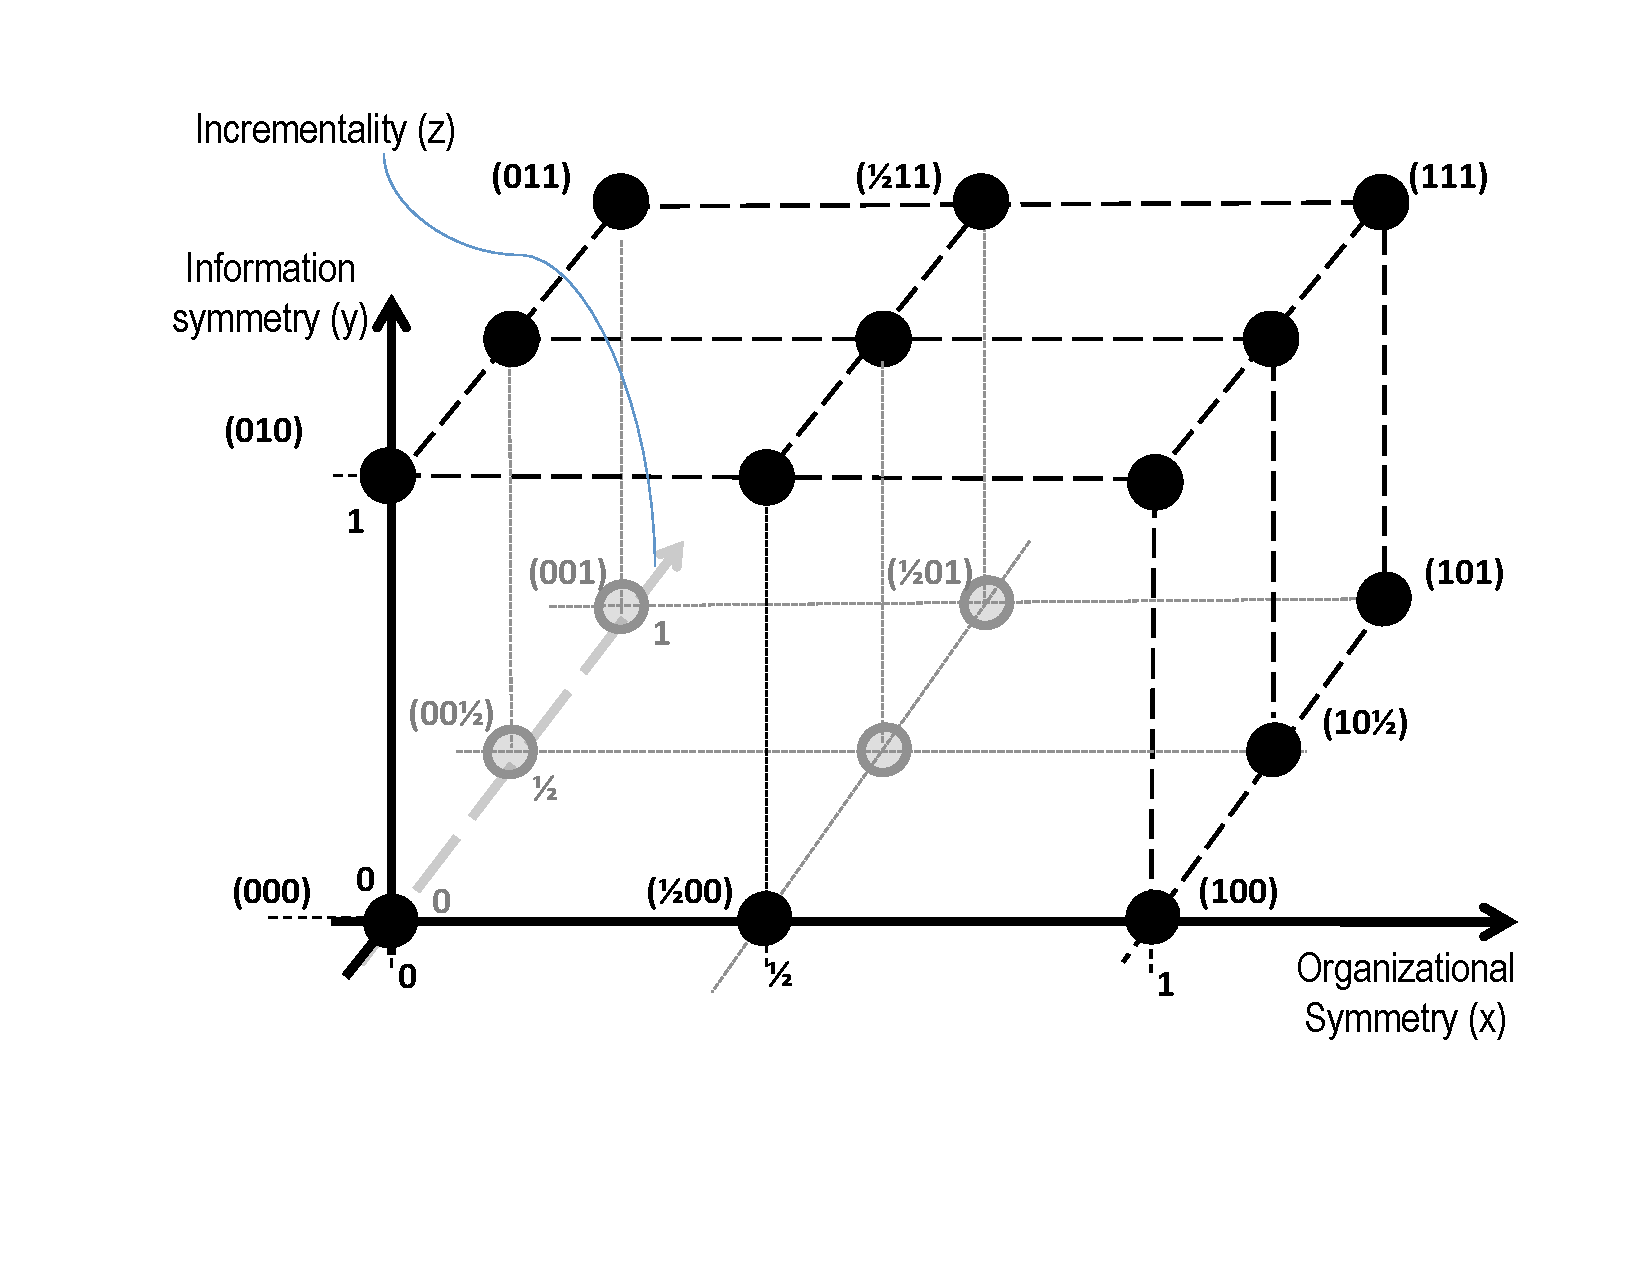
\includegraphics[width=100mm]{images/Synchronization-types}
\caption{3D dimension of Synchronization Scenarios}
\label{fig:SynchTypePic}
\end{figure}

%We later compare the concurrency aspect of the Synchronization with these three dimensions. We assume two model spaces(set of models) \textbf{A} and \textbf{B} and they are supposed to be aligned(consistent) w.r.t. a relation \textbf{R}. It should be mentioned that we assume the more common cases of synchronization which only two models are involved.

\subsubsection{Organizational Symmetry.} 
{\em Organizational Symmetry} represents how far we consider one side active in terms of accepting and propagating its changes during a synchronization scenario. This dimension captures synchronizer domain of application perspective in necessity of change propagation from one side to another side. For example synchronizer doesn't wish to allow any change propagation from A to B even if it is technically possible or not, e.g. in generation of object code from source code. we call this situation {\em Organizationally Asymmetric} or \textsf{org-symmetry=$0$}. In another word change propagation in this case is unidirectional and then one side would be always {\em passive} and the other side would be always {\em active}. As apposed to latter case, {\em Organizationally Symmetric} or \textsf{org-symmetry=$1$} means that change propagation is bidirectional and it is not prohibited from neither side, then both sides would be {\em active}. There is also some cases where some (and not all) changes from one side are allowed to be propagated. E.g., we prohibit tuple deleting propagation from the view to the source but letting tuple addition in view to be propagated to the source like the case we already discussed in previous section example. We call this type {\em Organizationally Semi-Symmetry} and show it by \textsf{org-symmetry=$\tfrac{1}{2}$}. According to the design decision of the synchronization framework implementation, change prohibition or making either side {\em active} or {\em passive}, can be implemented either by discarding the prohibited changes or by simply not allowing the user to do changes on models at first place. 


%--------------this part is cut out---------------
%(Because of the asymetry in the plain $info-symm \times Act.$  !!!!)
%------------I restricted the formalization of the act. dimension to some specific cases and tried to rewrite it in a new format--------
%
%We restrict the  \textbf{Formalization of Active-Passive Formalization} to Assymentric , non-incremental cases ({\em inc.=0, Inf.=0}) in this paper. You can find the full formalization of the case in (Cite to Tech report) \cite{Tech report}.
%
%We are extending the {\em Lenses} definition in Def. 1 by introducing two new functions $get^- $ and $gen^-$ which are inclusion of two functions $get$ and $gen$ respectively. These two functions leave out the prohibited domain of changes form the synchronization framework by restricting $get$ and $gen$ domains to acceptable ones.
% 
%\begin{ProposalDef}
%Let a lens $L^\leq_{0}=(M, M, get, put)$ is given. we define {\em asymmetric active-passive} cases as  $_{act}L^\leq_{0}=(M, N, get, put, get^-, gen^-) $  for $act \in \{0,1/2,1\}$ where $get^- \subseteq get$ and $,gen^- \subseteq gen$ as below:
%
%(a) $_{0}L^\leq_{0}$ is the case $(0,0,0)$ where $get^- = get$ and $gen^-=\emptyset$
%
%(b) $_{1 \over 2}L^\leq_{0}$ is the case $({1 \over 2},0,0)$ where $get^- = get \ and $ and $gen^- \subsetneq  gen$
%
%(c) $_{1}L^\leq_{0}$ is the case $(1,0,0)$ where $get^- = get \ and $ and $gen^- =  gen$
%
%
%\end{ProposalDef}
%
%we are defining $_{act}L^\geq_0: M \rightleftharpoons N$ as dual of above definition where {\em get} and {\em gen} are syntactically inter-replaced in (a),(b),(c). That is because of asymmetry in {\em info.} dimension ($ L^\leq$  vs. $L^\geq$). These asymmetries give rise to two cases for each point of $ inf.=0$ on the $act. \times Inc.$ plain. That is why we colored these point grey rather than black in Figure  \ref{fig:mt-space}
%
%Definition 5 can be generalized for the $dlt \in \{{1 \over 2},1 \}$ and {\em info.=1}.
%
%It is better to put the period table here as a summery. Something like this:
%
%------
%
%[Since we capture the user perspective (application perspective of synchronizer here, there is an space to capture some other aspects than Act. symmetry. for example we don't capture this idea how far we can tolerate inconsistency in two supposedly consistend models? (in another word what should be the granularity of the allowed change before we require alignment process happen) ]
%
%[The concept of \textbf {dependability} was not clear for me from what was written in the text, So I put down my understanding from this dimmension, that is why I call it \textbf{concurrency dimension} rather than Dependability
%
%------------cut out until here-------------


\subsubsection{Information Symmetry.} 
{\em Information Symmetry} dimension captures if two models are informationally symmetric or asymmetric. In {\em Information Asymmetric} or \textsf{inf-symmetry=$0$} case, one side existence informationally suffices to create the other side. In another word having one model, we can get the other one uniquely. This is the case in our example in previous section where \textsf{get*(A)} can be completely derived from \textsf{A} or gernerally in all typical cases of table-view scenarios \cite{Keller:1987fk, Johnson08amast}, where view contents is completely derivable from the corresponding table contents. As opposed to that, in \textsf{inf-symmetry=$1$} or {\em Information Symmetric} case neither A, nor B can be informationally derivable from each other. E.g. Class diagram and Sequence diagram, neither can be derived from each other uniquely. Another perspective of looking at this dimension is based on {\em private} and {\em shared} parts of each side. In {\em Asymmetric} one side has its own non empty {\em  private} and {\em shared} parts where the other side only consist of a {\em shared} part with its {\em private} part being empty. In {\em Symmetric} case, neither of {\em private} and {\em shared} parts of involved models are empty (ref. Figure \ref{fig:Private-Public}). The latter case is  the more general case of the synchronization scenarios in practice. It is possible that both {\em private} parts of each side be empty, this is called the {\em Informationally Bijective} case which can be considered as especial case of information symmetric case. In this case two models are informationally equal but differently represented. Later on in section \ref{sec:Problem} we will again discuss this concept of {\em private} and {\em shared} parts in more details as one of the intended contribution of PhD thesis.

%:Key private-shared Picture
 \begin{figure}[ht!]
\centering
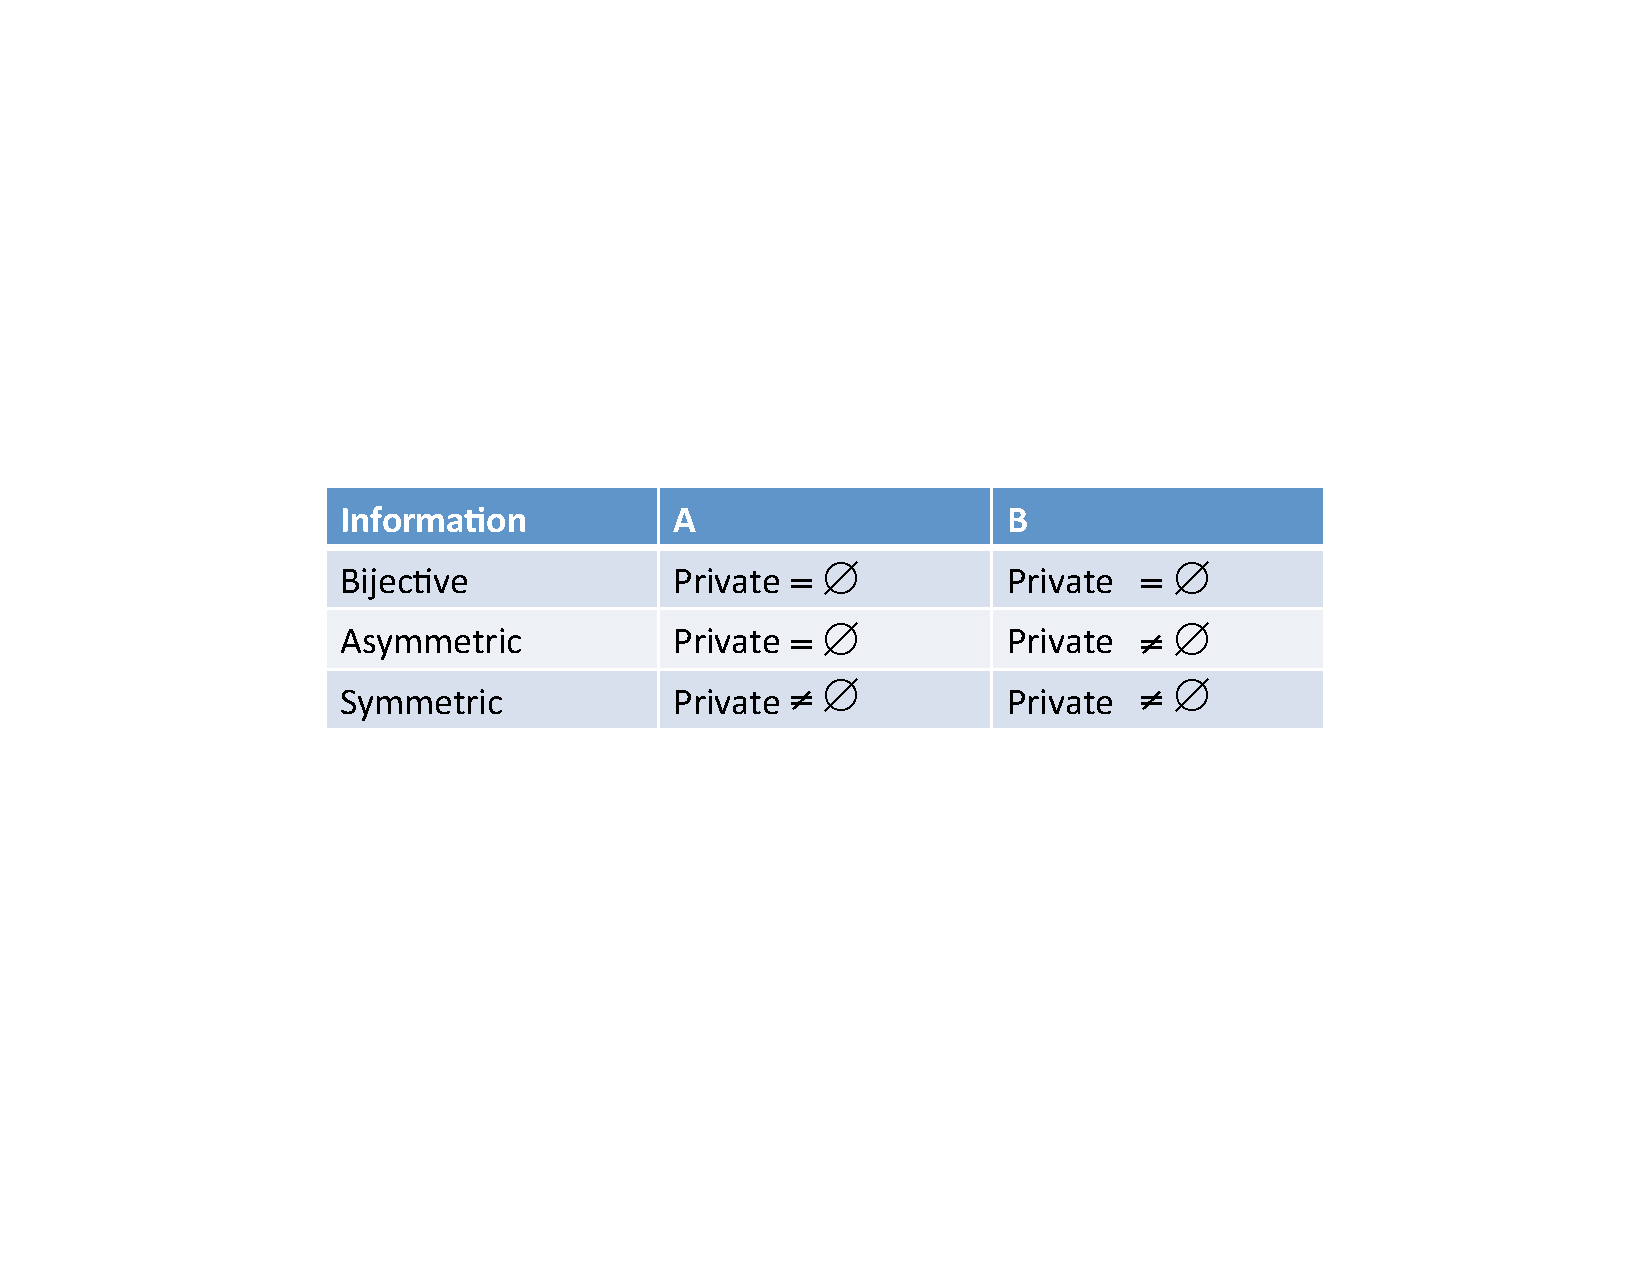
\includegraphics[width=100mm]{images/Private-Shared-Table}
\caption{private and shared parts in Information Symmetry dimension}
\label{fig:Private-Public}
\end{figure}

%a rough idea of defining a private part for Model A would be that, for any changes of the model B, you don't need to change private part to make both A and B consistent. But this idea need to be more invetigated in terms of Typed Attributed graphs.


\subsubsection{Incrementality.} \label{Incrementality} 
Synchronization scenarios can be classified into three cases in terms of maturity of its {\em Incrementality} method. These three categories are called {\em Batch-update}, {\em State-based} synchronization and {\em Delta-based} synchronization. In {\em batch update} or \textsf{inc=0}, one side is completely calculated from scratch whenever changes happen in another side. This naive strategy is not efficient at all in large model spaces $-$which are usually the case of synchronization application in practice, since for any even small changes on one side, considerable effort is imposed on the synchronization mechanism to calculate the other side. That is why it is usually used in small scale scenarios like type hierarchy update of Java codes \cite{antkiewicz2008:DesigndSpace}. if you take Models A and B again as both participants of the synchronization scenario, propagation function in this approach accepts  $A'$ (Changed $A$) as the mere input, and generates consistent $B'$ out of that from scratch. In comparison, \textsf{inc=$\tfrac{1}{2}$} or  {\em state-based} synchronizer takes $A'$ and $B$ as inputs, trying to calculate $B'$ where it is aligned with $A'$. This is far better than the previous case and usually is the intended scenarios when{\em Incremental synchronization} is mentioned in the literature. It is shown in \cite {Diskin:AsymmDelta:2011} that taking $A'$ and $B$ is not always enough in reconstructing the alignment between two models efficiently. So the more mature way of incrementally approach is providing the {\em Deltas}(Updates) as inputs $-$rather than just states, for the propagation function. we refer to the latter case as \textsf{inc=$1$} or {\em Delta-Based} synchronization. 

The way we choose $B'$ out of different alternatives in both {\em State-based} and {\em Delta-based} cases, is the subject which is discussed in more details as {\em minimal/least changes} in section \ref{sec:Problem} and is intended to be the other contribution in PhD thesis. That is also related to the {\em private} and {\em public} part identification too. Since for example it is desirable that the synchronizer doesn't change the {\em private} part of one side at all if we require the change become {\em minimal/least} on that side.



\subsubsection{Concurrency and its relation to other dimensions.} 
by {\em concurrent} synchronization we mean that two models are allowed to evolve concurrently. when we state that a synchronization is not {\em Concurrent}, it means mean that involved Models can not be changed simultaneously. In another word, supposing again Models A and B, if Model $A$ is evolving to $A'$ we first need to propagate its changes to $B$ and later on, evolution of Model $B$ would be allowed. In implementation it would mean that if even both models evolve simultaneously, we would give more importance on changes of one model which is termed as as {\em master}, while ignoring the changes of  the other, then is termed as {\em slave} and trying to make them aligned again. As apposed to that, in {\em concurrent} scenario, simultaneous changes to the models are allowed and both model changes are taken into consideration in the alignment process and non would be {\em slave}. The latter case is more desirable and the common scenarios in practice while it is more complicated than the former one, since the synchronizer needs to take into account both sides changes while trying to establish the alignment between them again. Though again in either case it is desirable to establish alignment by {\em minimal/least} changes application, the concurrent case add more complexity to {\em minimal/least} changes application by adding the necessity to consider both side simultaneously in the procedure. This is the third subject which will also be discussed in section \ref{sec:Problem} and is intended to be in the scope of the PhD thesis contribution to incremental model synchronization. 

%Orthogonality of the aforementioned three dimension in Figure \ref{fig:SynchTypePic} is somehow clear --{\em Information symmetry}, {\em Incrementality} and {\em Organizational symmetry} are orthogonal, since they are representing three independent aspect of the synchronization scenario. For each cases of information symmetric and asymmetric, and also for every case of {\em batch-update}, {\em state-based} update and {\em delta-based} update, we would have three possibility of organizational symmetry. Also being {\em Information symmetric}, {\em asymmetric} or {\em bijective} doesn't depend on the approach of the incrementality. But 

Concurrency is not orthogonal to aforementioned three dimensions. For example in \textsf{org-symmetry=0}, one side being {\em passive} would make the other side being always treated as {\em master} in non-concurrent cases, so making concurrent and non-concurrent cases identical. Another observation is that it seems being {\em passive} in terms of {\em Organizational Symmetry} differs from being {\em slave} in concurrent updates, since being {\em master} or {\em slave}, not necessarily fixed in non-concurrent case while being {\em passive} is a fixed parameter in {\em Organizational Symmetry} dimension .


%\hl { I would identify some problems like:
%
%Private and shared parts and minimal alignment.
%concurrency dimension its relation to info-symmetry and its formalization
%conflict resolution in concurrent updates. 
%
%}

%-------------------your writings  from paper--------
%\subsection{Concurrency Dimension ({\em Conc. Dimension})} capture the possibility of concurrent model evolution (models {\em co-evolution}) in the synchronization framework. Conc.=0 means that Models $A$ and $B$ can not be changed simultaneously. It means that if Model $A$ is evolving to $A'$ we need to first propagate its changes to $B$ and later on, evolution of Model $B$ would be allowed. In implementation it would mean that if even both models evolve simultaneously, we would give more importance on changes of one model and taking it as as $Master$ (say $A$), while ignoring the changes of the other(Say $B$) and trying to make them aligned again. In comparison,  in Conc.=1 case, simultaneous changes to the models are allowed and both models changes are taken into consideration in the alignment process. It means that synchronization framework tries to make the minimum changes possible on evolved Models $A'$ and $B'$ to produced the new aligned Models $A''$ and $B''$. The later case is more mature and the most desirable case of synchronization. We leave the formalization of this dimension for future works. [(We can write some examples here like state-chart and sequence diagram)]
%
%%:KEY  Orthogonality
%\subsection{Orthogonality of the Four dimensions}
%[better to describe orthogonality with one example]
%
%aforementioned four dimensions are orthogonal to each other and would built four axis of synchronization space giving rise to  ... types of synchronization scenarios. {\em Conc.} dimension is orthogonal to other three dimensions, because in each of them it adds two possibility of being concurrent (conc.=1) or not (conc.=0). For example it doesn't matter weather our incrementality be stat-based ({\em Inc.=1/2}) or delta-base ({\em Inc.=1}) or weather we have an information symmetric case({\em info.=1}) or asymmetric case ({\em info.=0}), in either case we can let concurrent updates happen or not. 
%Although one side being passive(act.=0) might make the other side to be always treated as {\em Master} in non-concurrent cases, so making all {\em conc.=1}  and {\em conc.=0} cases identical, for other cases of the {\em act.} dimension,  being concurrent or not gives rise to different synchronization types. i.e. \{ {\em act.=1/2,  conc.=0} \} and \{ {\em act.=1/2,  conc.=0} \} are two distinct cases of synchronization. That is because we believe being {\em passive} differs from being {\em slave} in concurrent updates, since choosing one side to be master or slave is not fixed in {\em conc.=0} while being passive is the parameter which is fixed throughout synchronization scenario.  {\em Inc.} dimension is also orthogonal to other two dimensions: {\em Info.} and {\em act.}, since no matter if we have information asymmetric case or symmetric case, and whichever side be {\em active} or {\em passive}, we can treat each case independently either in {\em batch-update} approach, {\em state-base} approach or {\em delta-base} approach. How far one side be active is again independent of weather it is information symmetric or asymmetric case. 
%
%
%---------------------







\subsection{Pair of Transformers and Bidirectional Transformation Languages}
In model synchronization, changes propagation is usually applied by execution of a pair of transformers which we call {\em forward} and {\em backward} transformers or propagation functions. These transformers as we will discuss in next section are necessary to be treated as a pair of functions which satisfy some properties. 
When we transfer one model(say Model A) to another model(say Model B) by {\em forward} transformation function, we usually desire to have a {\em backward} counterpart which transfers B to A. 

Suppose that A and B are consistent if they satisfy the constraints defined by a relation $R$
% between $A$ and $B$ as a set of Models
%, and {\em Pair of Transformers}({\em forward} and {\em backward})  which are in accordance with this Relation\footnote{\label{note1}By in accordance we mean holding some properties like {\em Correctness}, {\em Completeness} and etc. which is defined later. {\em Correctness} property is necessarily basic one and should hold for all pairs of transformers.}
. Often in practice R is not explicitly defined and just the transformers is defined using some transformation languages. For example languages like {\em ATL} \cite{Jouault:2008:ATL}, {\em Viatra2} \cite {Balogh:2006:Viatra2}, {\em QVT-O} \cite{OMG:QVT:2011} or even Regular programming languages like {\em Java} are used for writing transformers. In these situations getting a backward transformation is not trivial and oftentimes requires the user to code the backward transformation separately by hand. It is often desirable that these {\em forward} and {\em backward} transformers be consistent \footnote{\label{note1}holding some properties like {\em Hippocraticness}, {\em Undoability} and etc., which is discussed later } \cite{Diskin:DeltaSymm2011kl, Foster:LensCombinators:2005tg, steven:QVT-Semantic2010}, but maintaining the consistency in pair of transformers which is separatly coded by user is not easy and straight forward. That is why the concept of the {\em Bidirectional Transformation Languages(BX)} in which {\em consistent} transformers can be extracted automatically out of one (forward) specification is emerged. This specification in {\em BX} is somehow more explicitly specifying the relation R between A and B. For example {\em QVT-R} \cite{OMG:QVT:2011}, {\em Triple Graph Grammars(TGG)} \cite{Schurr:1995:TGGIntro}, {\em Lenses} Framework \cite {Foster:LensCombinators:2005tg} and {\em GroundTram} \cite{hidaka2011:Groundtram} frameworks are providing {\em BX} facility. From the aforementioned frameworks, only TGG works on TAG\footnote{ refere to Definition \ref {Def:TAG}}. Table below summarizes the datastructure each of these languages support for model representation:


%:Key BX Framework Table representation
\begin{center}
\begin{tabular}{|c|c|}
\hline 
\textbf{Framework} & \textbf{Model Representation}\tabularnewline
\hline 
\hline 
QVT-R & UML Meta-Model\tabularnewline
\hline 
TGG & Typed Attributed Graph\tabularnewline
\hline 
GroundTram & Labeled Graph\tabularnewline
\hline 
Boomerang & String\tabularnewline
\hline 
\end{tabular}
\end{center}

Although having BX is desirable but in theory and practice there are some obstacles in making them applicable: (1)Semantic of extracting a consistent backward transformation is not trivial, (2)There doesn't exist yet a rule of thumb what is the appropriate collection of properties for the pair of transformers in different application domains (ref. \ref{Synch:Prop}) (3)Specifying transformers as one specification in BX languages like QVT-R is more complicated and trickier than writing the same transformer in one-directional transformation languages.
Whatever approach we take for specifying the synchronizer transformers, they are required to satisfy some properties which we will discuss in the following section.

%Out of aforementioned frameworks for the BX, each one has its pros and cons, but non is yet gained the maturity enough to be widely used in industrial cases. \hl{Out of those, since TGG are supporting TAG, we will discuss that in .... in more detail and will examine its specifications in Sec...}
%
%\hl{(You can Write a section on TGG and formally define it and discuss it formally and say its strenghes and weeknesses)}
%
%Now write down properties name and define them:

\subsection{Consistency properties of transformers}
It is desirable that pair of transformers(forward/backward) satisfy some consistency properties. For Example {\em Correctness} of the transformers is the rudementary requirement which insures that transformers operate correctly. Other consistency properties like {\em Completeness}, {\em Hippocraticness}, {\em Undoability} and {\em Invertability} are also discussed in this section. When we talk about model {\em Synchronization} we desire that the corresponding transformers become consistent, where the consistency of the transformers is defined as conforming to subset of the following properties depending on the domain of the synchronizer application. First we define the Correctness property.
\subsubsection{Correctness.}
\label{Synch:Prop}
%We define the notion of the Correctness in a abstract way here, and later on we would make it concrete for each of the types specified in Section \ref{subsec:SynchScen}. 
Let's call {\em forward} and {\em backward} transformers $\overset{\rightarrow}{R}$ and $\overset{\leftarrow}{R}$ consequently supposing that they are total functions, and suppose that Relation $R$ is a desirable relation between two set of models or meta-models, $A$ and $B$. {\em Correctness} property as it is expected, simply ensures that a pair of  transformers are functioning correctly.

%:Key Correctness
\begin{ProposalDef} \label{CorrectnessDef}
A pair of transformers  ($\overset{\rightarrow}{R}$, $ \overset{\leftarrow}{R}$) are \textbf{Correct} w.r.t. $R \subseteq A\times B$, if  $(a,\overset{\rightarrow}{R}(p_1)) \in R$ and $(\overset{\leftarrow}{R}(p_2),b) \in R$ where $p_1$ and $p_2$ are set of input parameters.
$p_1$ for {\em Batch-update}, {\em State-based} and {\em Delta-based} cases(ref. \ref{sub:synchSpace}) are $\{b\}$, $\{a,b\}$ and $\{\Delta a,b\}$ consequently where $a,a' \in A, b \in B$ and $\Delta a=(a,\Delta,a')$ for $\Delta $ being a mapping between elements of $a$ and $a' $.  $p_2$ is defined the same way as $p_1$ if we interchange $a$ and $b$ in $p_1$. 
\end{ProposalDef}
This property is defined in \cite{steven:QVT-Semantic2010} and \cite{Diskin:AsymmDelta:2011} for {\em Information Symmetric} and {\em Delta-based} case. In \cite{Bohannon:2008:Boomerang,Hofmann:2011:SymLens} this property is defined for {\em Information Asymmetric} and {\em State-based} Cases.  

\subsubsection{Hippocraticness, or �check-then-enforce�.} 
This property states that the transformers should not cause any change if two models are already consistent w.r.t. R. 
 
 %:Key Hippocratic
\begin{ProposalDef}
A pair of transformers  ($\overset{\rightarrow}{R}$, $ \overset{\leftarrow}{R}$) are \textbf{Hippocratic} w.r.t. $R \subseteq A\times B$, where  $\forall a \in A$ and $\forall b \in B$: if $(a,b) \in R$  then $\overset{\rightarrow}{R}(p_1)=b$ and $(\overset{\leftarrow}{R}(p_2)=a)$
\end{ProposalDef}

$p_1$ and $p_2$ are defined like Definition \ref{CorrectnessDef}. This property is one of the requirements of the QVT-R specification in OMG standard \cite{OMG:QVT:2011}

\subsubsection{Undoability.}
Undoability is introduced by Steven in \cite{steven:QVT-Semantic2010}. That means if we undo the changes of the $A$, any changes that happened on $B$ because of synchronization, should be rolled back to exactly its original state. We define this property for {\em State-Based} scenario as we would see it is trivial for {\em Batch-Update}. 

\begin{ProposalDef}
A Pair of Transformers  ($\overset{\rightarrow}{R}$, $ \overset{\leftarrow}{R}$) are \textbf{Undoabe} w.r.t.  $R \subseteq A\times B$, where  $\forall a,a' \in A$ and $\forall b,b' \in B$: if $(a,b) \in R$  then $\overset{\rightarrow}{R}(a, \overset{\rightarrow}{R}(a',b))=b$ and $\overset{\leftarrow}{R}(\overset{\leftarrow}{R}(b',a),b))=a$ 
\end{ProposalDef}

For the {\em batch-update} case this property is trivial and holding all the times, since we assume that the transformers are functions, then rolling back $a'$ to $a$ and executing the $\overset{\rightarrow}{R}$ on that we are obviously expecting to get $b$ again. However according above definition this might not be the case for the {\em State-based} or {\em Delta-basd} scenarios.

It is arguable that this property is suitable to be imposed on the synchronization implementation environment rather than the synchronization transformers.  Since at the moment {\em undoability} is well supported by modelling environments, while we believe imposing this property on transformers sometimes might be more restrictive.

\subsubsection{Invertability.}
It is informally means that starting from one model and going forward and backward by transformers, we will end up with the same model. In another word it states that the {\em forward} and {\em backward} transformers are the inverse of each other and functioning in reverse directions. We define invertability for the {\em State-based} cases. the definition can be easily extended for the other synchronization scenarios. Following definition is adopted from \cite{Zinovy:2008:AlgForSynch}.

\begin{ProposalDef}
A pair of transformers  ($\overset{\rightarrow}{R}$, $ \overset{\leftarrow}{R}$) are \textbf{Invertabe} w.r.t.  $R \subseteq A\times B$, if  $\forall a,a' \in A$ and $\forall b,b' \in B$:  $\overset{\rightarrow}{R}(a, \overset{\leftarrow}{R}(a,b',b),b)=b'$ and $\overset{\leftarrow}{R}(b, \overset{\rightarrow}{R}(a,a',b),a)=b'$ where $\{(a,b),(a',b')\} \subseteq R$ 
\end{ProposalDef}


\subsubsection{Completeness.}
Completeness says if there exists at least one model, say $b$, which is in relation with model $a$, then transformer should be able to transform $a$ to it. In another word {\em Completeness} states that the transformers should be total functions and return nonempty in the case there is a counterpart for its input(s) regarding relation R


\begin{ProposalDef}
A pair of transformers  ($\overset{\rightarrow}{R}$, $ \overset{\leftarrow}{R}$) are \textbf{Complete} w.r.t.  $R \subseteq A\times B$, if $\forall a \in A,  \overset{\rightarrow}{R}(a)\neq \emptyset$ if $\exists b \in B$ where $(a,b) \in R$  and if $\forall b \in B,  \overset{\leftarrow}{R}(b)\neq \emptyset$ if $\exists a \in A$ where $(a,b) \in R$ 
\end{ProposalDef}


%Typed Attributed Graph Definition
\subsection{Models as Typed Attributed Graphs}
\label{sub:TAG}
As we mentioned in previous section, different languages in synchronization and transformation environments, support various data structure for model representation. Out of those, Typed Attributed Graph(TAG) is known to subsume other data structure in terms of being more expressive in models formal representation. for example the meta-model concept can not be well expressed in labeled Graphs while we would see it has a clear definition in terms of TAG.

In general a model can be represented as a graph consisting of a nodes and edges. E.g. a Class diagram in UML is a graph with classes as nodes and associations between them asedges. Since we need a richer structure than a simple graph we need to extend the formality of a graph to make it possible to capture further values annotated to the nodes and edges, Hence {\em attributed graphs} are introduced. Attributed graphs are like ordinary graphs extended in a way that for every {\em node} and {\em edge}, it is possible to introduced a data called  {\em attribute} and bind that by an edge called {\em attribute edge} to corresponding nodes and edges. So, first we need to extend the concept of regular graph to make it possible for edges to have outgoing edges like nodes. This extended version of graphs is called {\em E-Graph} and introduced in the following.


%:Key Def1(E-graph G)
\begin{ProposalDef}
An \textbf{E-graph G} is defined as $G=(V_G,E_G, V_D, E_{NA},E_{EA} ,(source_j$ $,target_j)_{j \in \{G,NA,EA\}) }$
\begin{itemize}
	\item $(V_G,E_G,source_G,target_G)$ constitutes a regular Graph with $V_G$ as Nodes, $E_G$ as Edges and $source_G$ and $target_G$ as source and target functions  respectively.
	\item $V_D$ is a Data Nodes
	\item $E_{NA}$ and $E_{EA}$ are called Node Attributes and Edges Attributes, which are connecting respectively $V_G$  and $E_G$ to $V_D$. 
	\item source and target functions are defined as below:
	\begin{itemize}
		\item $source_G : E_G \rightarrow V_G$, $targetG : E_G \rightarrow V_G$;
		\item $source_{NA} : E_{NA} \rightarrow V_G$, $target_{NA}: E_{NA} \rightarrow V_D$;
		\item $source_{EA} : E_{EA} \rightarrow E_G$, $target_{EA}: E_{EA} \rightarrow V_D$;
	\end{itemize}
\end{itemize}

\end{ProposalDef}

%:Key Def2(morphism between E-graphs)
\begin{ProposalDef}

\textbf{morphism between E-graphs} $G^1$ and $G^2$ with 
$G^k = (V_G^k, V_D^k, E_G^k, E_{NA}^k$ $,E_{EA}^k, (source_j^k, target_j^k)_{j \in \{ G, NA, EA \}})$ for $k = 1, 2$ is defined as $f:G^1 \rightarrow G^2$ which is a tuple $(f_{V_G},f_{V_D},f_{E_G},f_{E_{NA}},f_{E_{EA}})$ 
with $f_{V_i} : V_i^1 \rightarrow V_i^2$ and  $f_{E_j} : E_j^1 \rightarrow E_j^2$ for $i \in \{G,D\}$, $j \in \{G,NA,EA\}$ such that $f$ commutes with all source and target functions, for example $f_{V_G}  \circ source_G^1= source_G^2 \circ f_{E_G}$

\end{ProposalDef}

%:Key Def3(Category EGraphs)
\begin{ProposalDef}
E-graphs and E-graph morphisms form the \textbf{Category EGraphs}.
\end{ProposalDef}

 {\em Attributed Graphs} are Graphs that is accompanied by a Data Algebra in a sense that the Data Nodes are taken from the subset of algebra {\em Carrier sets}. To be more precise, we first distinguish a subset of a Carrier set of an algebra and consider the contents of each member in this subset as a {\em Data Node}. In graphical illustration of the Attributed Typed Graph we ignore those {\em Data Nodes} that are not reachable from the underlying graph nodes and edges. See an example in \cite{book:Ehrig2010} for more details.
  
%:Key Def4 (Att Graph Def)
\begin{ProposalDef}
Let $D_{SIG} = (S_D,OP_D)$ be a data signature with attribute value sorts $S_D$ and operations $OP_D$ and take $S'_D \subseteq S_D$. An \textbf{Attributed Graph(AG)} $AG = (G,D)$ consists of an E-graph $G$ together with a $D_{SIG}$-algebra $D$ such that $V_D$ is disjoint union of the selected carrier sets, i.e. $V_D=\overset{\centerdot}{\cup}_{s \in S'_D} D_s$ where $D_s$ is coresponding carrier set of s.
\end{ProposalDef}

%:Key Def5 (Att Graph Morphism )
\begin{ProposalDef}
an \textbf{Attributed Graph Morphism}  $f : AG^1 \rightarrow AG^2$ for two AG graphs $AG^1=(G^1,D^1)$ and $AG^2 = (G^2,D^2)$ is a pair $f=(f_G,f_D)$ with an E-graph morphism $f_G : G^1 \rightarrow G^2$ and an algebra homomorphism $f_D : D^1 \rightarrow D^2$ such that diagram (1) commutes for all $s \in S'_D$, where vertical arrows are inclusions:

\begin{figure}[ht!]
\centering
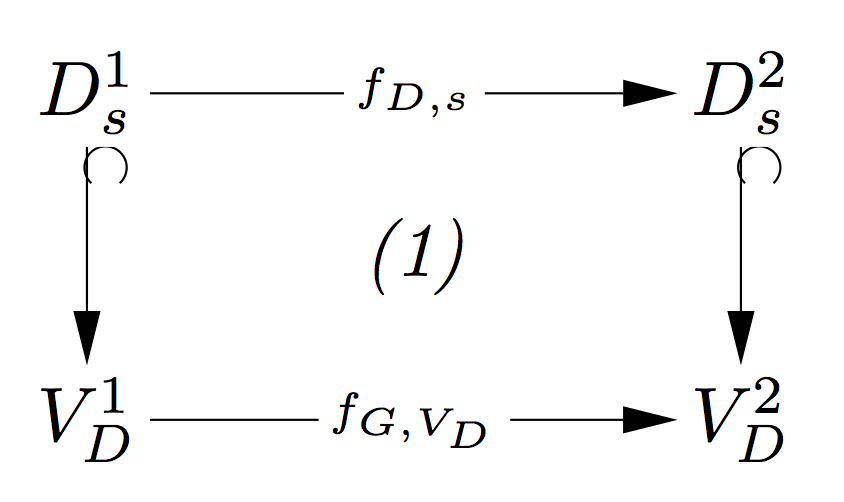
\includegraphics[width=50mm]{images/AGmorphism.png}
%\caption{AG }
\label{AG morphism}
\end{figure}

\end{ProposalDef}

For defining the Typed attributed Graph we need to first define the concept of final $D_{sig}$-algebra for a given algebra. final $D_{sig}$-algebra for an algebra is mapping somehow the name of the sort as a set to the sort as its interpretation. So cardinality of the interpreted sorts would be 1 for all of them. It maps the constant symbol of sort $S_i$, to the singleton member of corresponding carrier set $Z_{S_i}$, and following that, interpret the result of a function application on carrier set to the corresponding singleton member of the result sort.  
%:Key Def6 (final D_sig-Algebra)
\begin{ProposalDef}
Given a signature $SIG = (S, OP)$ , the \textbf{final $SIG$-algebra Z} is defined by $Z=(S_z, C_z, OP_z)$ where:

\begin{itemize}
	%\item $S_z = D_k$ where  $D_k=\{k\}$ for each sort $k \in S$;
	\item $S_z = D_s$ where  $D_s=\{s\}$ for each sort $s \in S$;
	%	\item $C_z = s \in Z_s$  for a constant symbol $c_s: \rightarrow s \in OP$;
	\item $C_z = k \in D_s$  for a constant symbol $c_s: \rightarrow s \in OP$;
	%\item $op^I : \{s_1\} \ldots  \{s_n\} \rightarrow \{s\} : (s_1 ... s_n) \mapsto s$ for each operation symbol $op:s_1 ... s_n \rightarrow s \in OP$
	\item $OP_z : \{s_1\} \ldots  \{s_n\} \rightarrow \{s\} : (s_1 ... s_n) \mapsto s$ for each operation symbol
$op:s_1 ... s_n \rightarrow s \in OP$
 \end{itemize}

\end{ProposalDef}


%%:Key Def6 (Typed Att Graph)
%\begin{ProposalDef}
%an \textbf{Attributed Graph Morphism}  $f : AG^1 \rightarrow AG^2$ for two AG graphs $AG^1=(G^1,D^1)$ and $AG^2 = (G^2,D^2)$ is a pair $f=(f_G,f_D)$ with an E-graph morphism $f_G : G^1 \rightarrow G^2$ and an algebra homomorphism $f_D : D^1 \rightarrow D^2$ such that diagram (1) commutes for all $s \in S'_D$, where vertical arrows are inclusions:
%
%\begin{figure}[ht!]
%\centering
%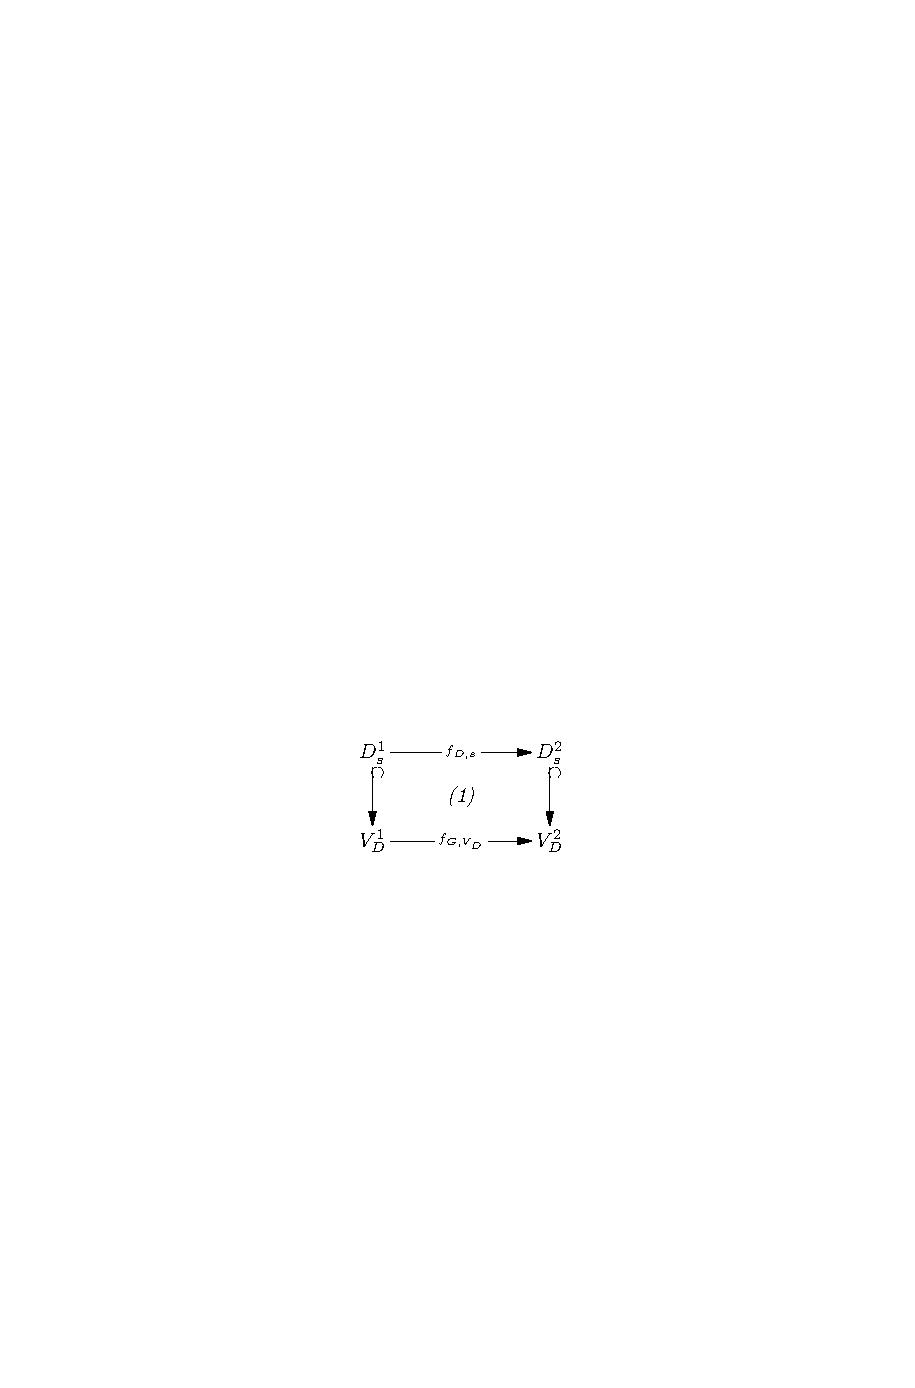
\includegraphics[width=60mm]{images/AG-morphism}
%%\caption{AG }
%\label{AG morphism}
%\end{figure}
%
%\end{ProposalDef}

%:Key Def (Attributed Type Graph(ATG))
\begin{ProposalDef}
Given a signature $SIG = (S, OP)$ , an \textbf{Attributed Type Graph(ATG)} is an attributed graph $ATG=(TG,Z)$ where Z is the final $SIG$-algebra. 
\end{ProposalDef}

So for having an Attributed Type Graph as a Type of another Attributed Graph, we need to somehow specify the typing of the 
Attributed Graph Data Structure(Data Algebra) too. That is why we need to define a final $Sig$-algebra. Typing of the Attributed Graph Data Structure is represented by the final $SIG$-algebra of the corresponding Data Signature. In the following we define Typed Attributed Graph (TAG).

%:Key Def (Typed Attributed Graph)
\begin{ProposalDef}
\label{Def:TAG}
A \textbf{Typed Attributed Graph(TAG)} over $ATG$ is defined as $(AG, t)$  where $AG$ is an attributed graph and $t$ is an  attributed graph morphism from $AG$ to $ATG$
\end{ProposalDef}


Please observe that the data-signature of of the Attributed Type Graph and Typed Attributed Graphs, Typed over that would be the same, as the definitions above implies.

\begin{ProposalDef}
A \textbf{TAG morphism} between $TAG^1=(AG^1,t^1)$ and  $TAG^2=(AG^2,t^2)$ i.e. $f: TAG^1 \rightarrow TAG^2$ is an Attibuted Graph Morphism(AGT morphism) $f: AG^1 \rightarrow AG^2$ such that $t^2 \circ f=t^1$:
\end{ProposalDef}

\begin{figure}[ht!]
\centering
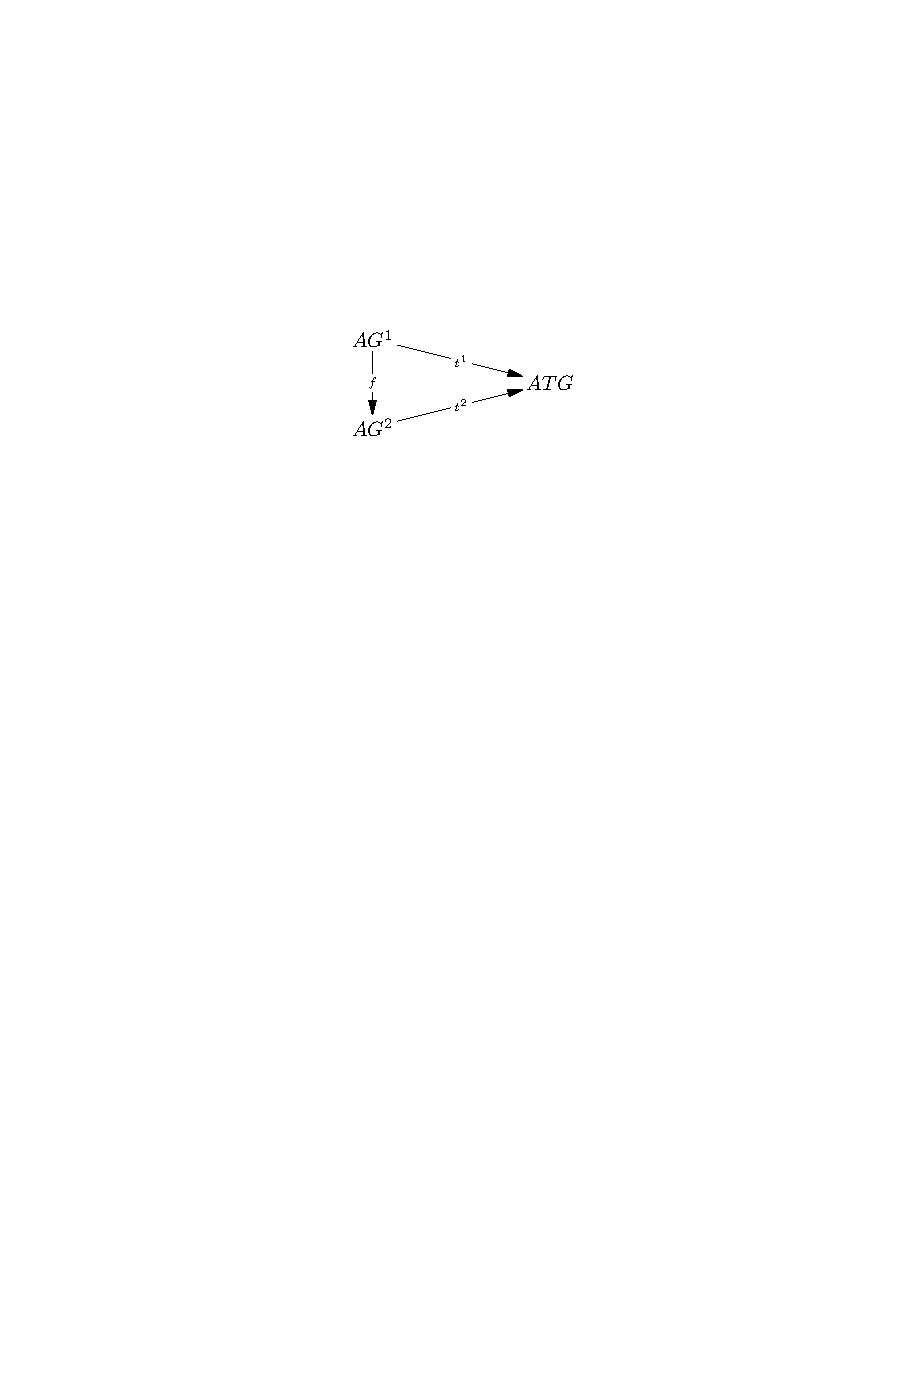
\includegraphics[width=50mm]{images/TAG-morphism}
%\caption{AG }
\label{AG morphism}
\end{figure}

In terminology of the Software Engineering, {\em Models} are equal to {\em Typed Attributed Graphs} and {\em Meta-Models} are equal to {\em Attributed Type Graphs}. This can be extended to more than one level, while meta-meta-model would be Attributed Type Graph for Attributed Type Graph of its beneath level as a Type. We should observe that all the {\em Entities} (Including Models, Meta-Models and Meta-Meta-Models) are Attributed Graphs, and the Data-signature of the connected {\em entities} by typing association(Typing Mapping) would be the same. In another word data-signature of the Model, Meta-Model and Meta-Meta-Model, all, would be the same.

\section{Problem Definition}
\label{sec:Problem}
We are going to discuss three issues regarding the synchronization scenarios: {\em Private} and {\em Shared} part identification, {\em Minimal/Least} change application and {\em Concurrent} synchronization. These three issues are somehow related to each other as we will discuss it. We are going to explain each issue in more details in the following. 

%and will try to refer to an example if it is necessary to more clarify the problem.

\subsubsection{Private and Share Parts.}
When some changes happens in one of the two related models, there are three ways to react: (1) changes are discarded (2) changes doesn't need to be propagated (3) changes impose changes to model counterpart and should be propagated.

choosing each of above options depends on the value of the synchronization type on {\em Organizational} axis: if it is {\em Asymmetric}, {\em Partial Symmetric} or {\em Symmetric.} Suppose that we define the case as organizationally  symmetric and incremental like in Figure \ref{fig:Example04}.  The main question is how we can distinguish which changes on Model B will  impose necessary changes on Model A and Which don't? The general definition of the {\em private} and {\em shared} part is based on the change propagation necessity. By {\em private parts} of the Model B, we mean the entities that any change to them would not impose changes to Model A to restore consistency,  as apposed to {\em shared parts} which any changes to them requires some changes on Model A to satisfy the constraints and  establish the consistency relation again (ref. Figure \ref{fig:private-shared}), So our later question would be ``what are the {\em private} and {\em shared} parts of the Model B?'' 

In practical implementation of the synchronization types (Figure \ref{fig:SynchTypePic}), the later definition of the private/shared part is not so useful and we need a kind of mechanism to distinguish the private/shared part before execution of the transformation function or alignment procedure to decide weather the type of the changes are private or shared, and based on that trigger the alignment procedure or not. This is important to know, since otherwise we will require that with any changes to the model we transform the whole model -- which is very costly, not efficient and time consuming in real application.
  
In the case of the example in section \ref{sub:example}, it seems that distinguishing the {\em private/shared} part can be based on the relation definition. E.g. we can say that \verb+from, to+ and \verb+time+ are shared parts of the Model B and the \verb+plane+ and \verb+fnum+ are the private parts. This seems to be known out of the relation definition syntax where if we see the names of entities in the relation definition, it would be considered as the {\em shared part} and otherwise it would be {\em private}. Even in the case of the flight price in model B, we can include it in the shared part.

%:Key Private and Shared part Picture
 \begin{figure}[ht!]
\centering
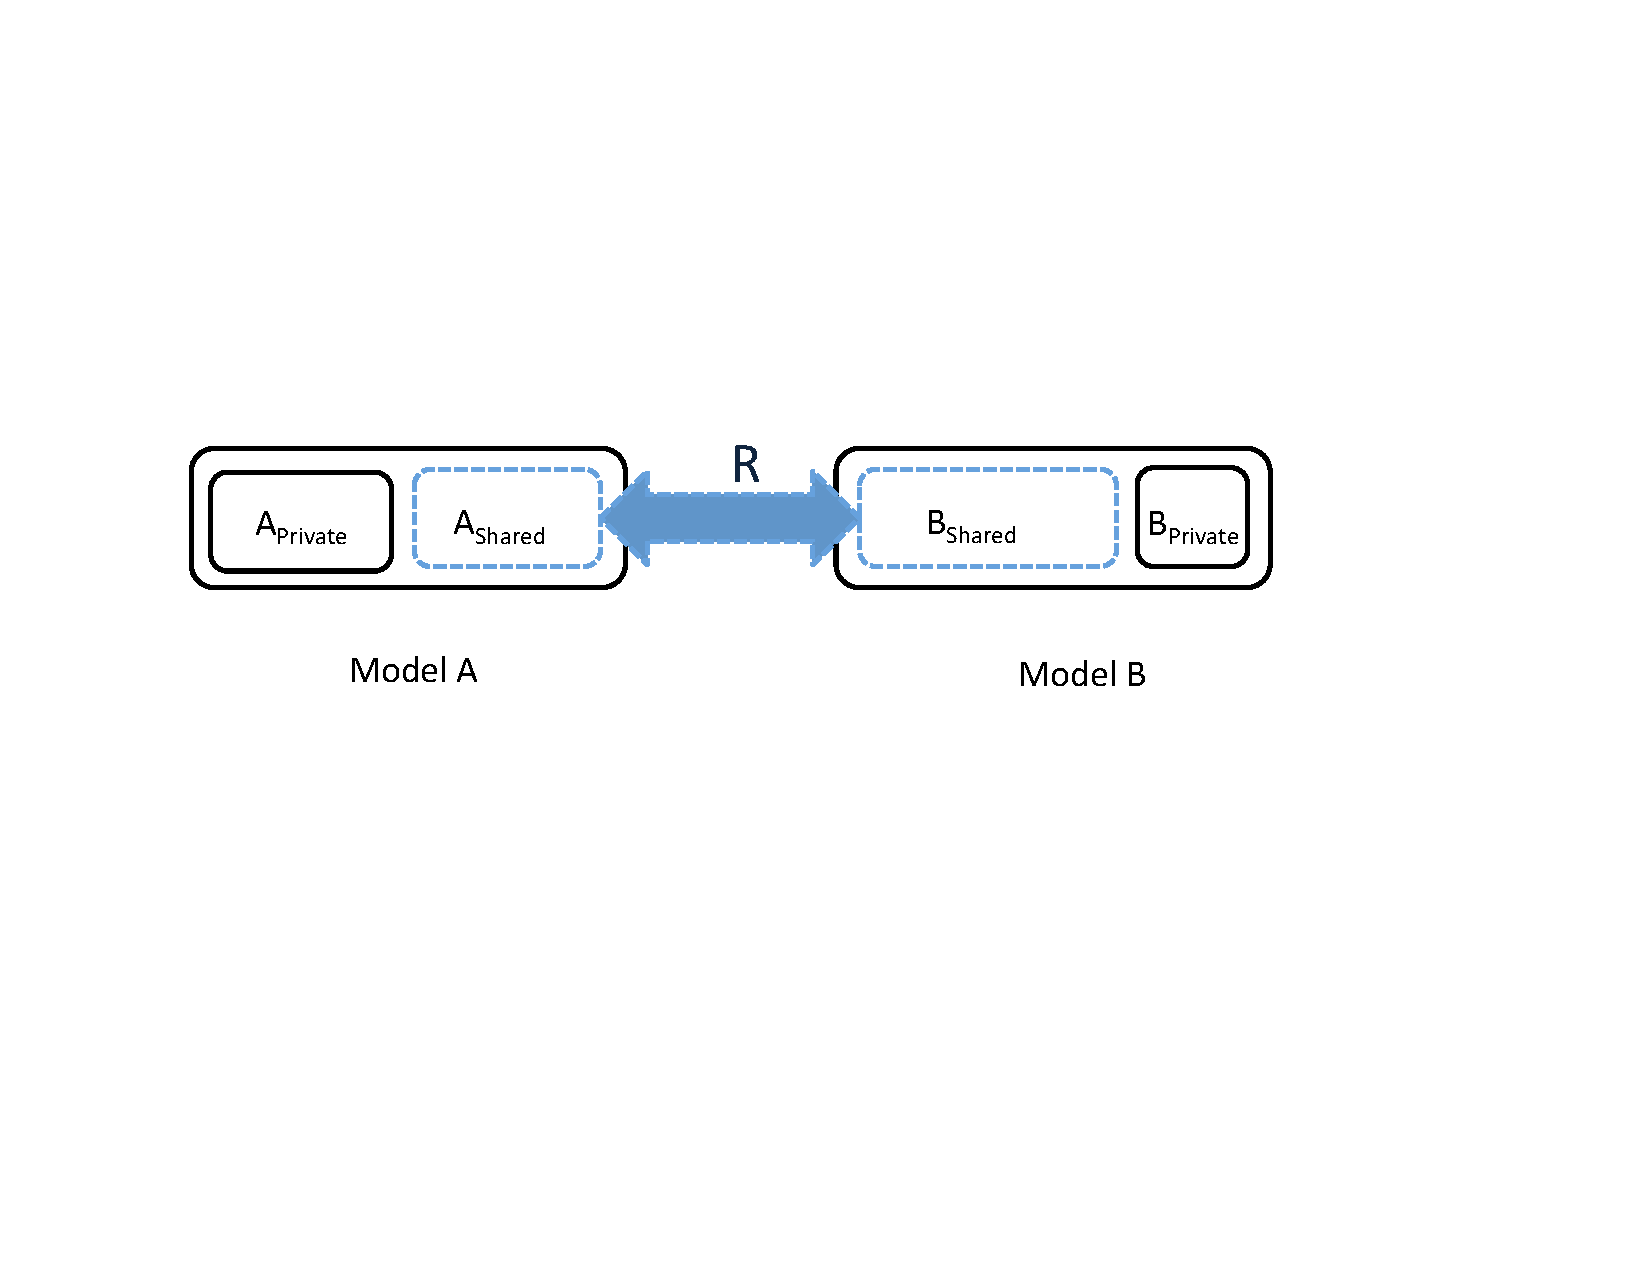
\includegraphics[width=100mm]{images/private-shared}
\caption{Each Model is consisting of Private/Shared parts}
\label{fig:private-shared}
\end{figure}

That is though seems somehow working in above example, there are two points it is necessary to mention out regarding that method: (1) Models in general sense are Typed Attributed Graphs(ref. section \ref{sub:TAG}) and the way the relation is defined among them in practice are not always like declarative mathematical relations. i.e. in some more popular transformation languages  like ATL \cite{Jouault:2008:ATL} and Viatra2 \cite{Balogh:2006:Viatra2} (non-BX), the relation is defined as functions and in some approaches like Triple Graph Grammars(TGG) \cite{Ehrig:2007:IPB:TGGFromalDef, Konigs:2006:TGGFormalDefSetBased}, the relation definition is operational rather than being declarative. Furthermore the notion of the functional dependancy, which is necessary in distinguishing the shared parts in simple models like database tables-- those entities functionally dependent to shared parts are also belong to shared parts (transitive closure) --   need to be generalized to the cross cutting constraints between the model elements inside the Graph of Model, which needs more investigation and study. It is also important to clarify how these private/shared parts granularity is defined based on the TAG entities: nodes, edges, or attributes or combination of them  (ref. TAG definition in \ref{sub:TAG})(2) The more we can precisely distinguish the boundaries of the private part, the more efficient and less costly would be our synchronization alignment procedure. The worse extreme safe case is to take the whole model B being shared, so triggering the alignment procedure in any changes which occurs on Model B which is far away from being optimal technique.

\subsubsection{Minimal/Least change application in model alignment.}
suppose we have the case of \textsf{Inc.=$\tfrac{1}{2}$ or $1$} and \textsf{org-symm.=1}, and we want to propagate the synchronization from Model B to Model A. Again you can take the example in Figure \ref{fig:Example04} into account and suppose the update is changing the price of the flight in Model B from 50 to 200. Remember that the flight price in Model B should be at least \$100 less than the model A. we assume that we already identified the price in model B as a private part-- So we already need to know about private and public parts. The question would be ``what would be the changes on the corresponding flight in Model A when we change the price from 50 to 200 in Model B?'' The answer here seems to be simple. According to price constraint, we increase the corresponding flight price in Model A up to the extend that make it 150 plus the flight price in Model B. But why not we increase the flight price to $300+10$ or $300+20$. Either of these changes would result in a consistent Model with Model B. The thing is that from synchronizer perspective it doesn't matter if we make the flight price in model A \$300, or 10, or 20 dollar or $X$ dollar more! (ref. Figure  \ref{fig:leastChange}) But it seems that some range of options are more desirable than the others in the sense that they change model A to the nearest model $A'$ where they can establish again the alignment. In Our example we can say that this is an increase of price up to the price of the Flight plus 100, is the least change in Model A. 

%:Key leastChange Picture
 \begin{figure}[ht!]
\centering
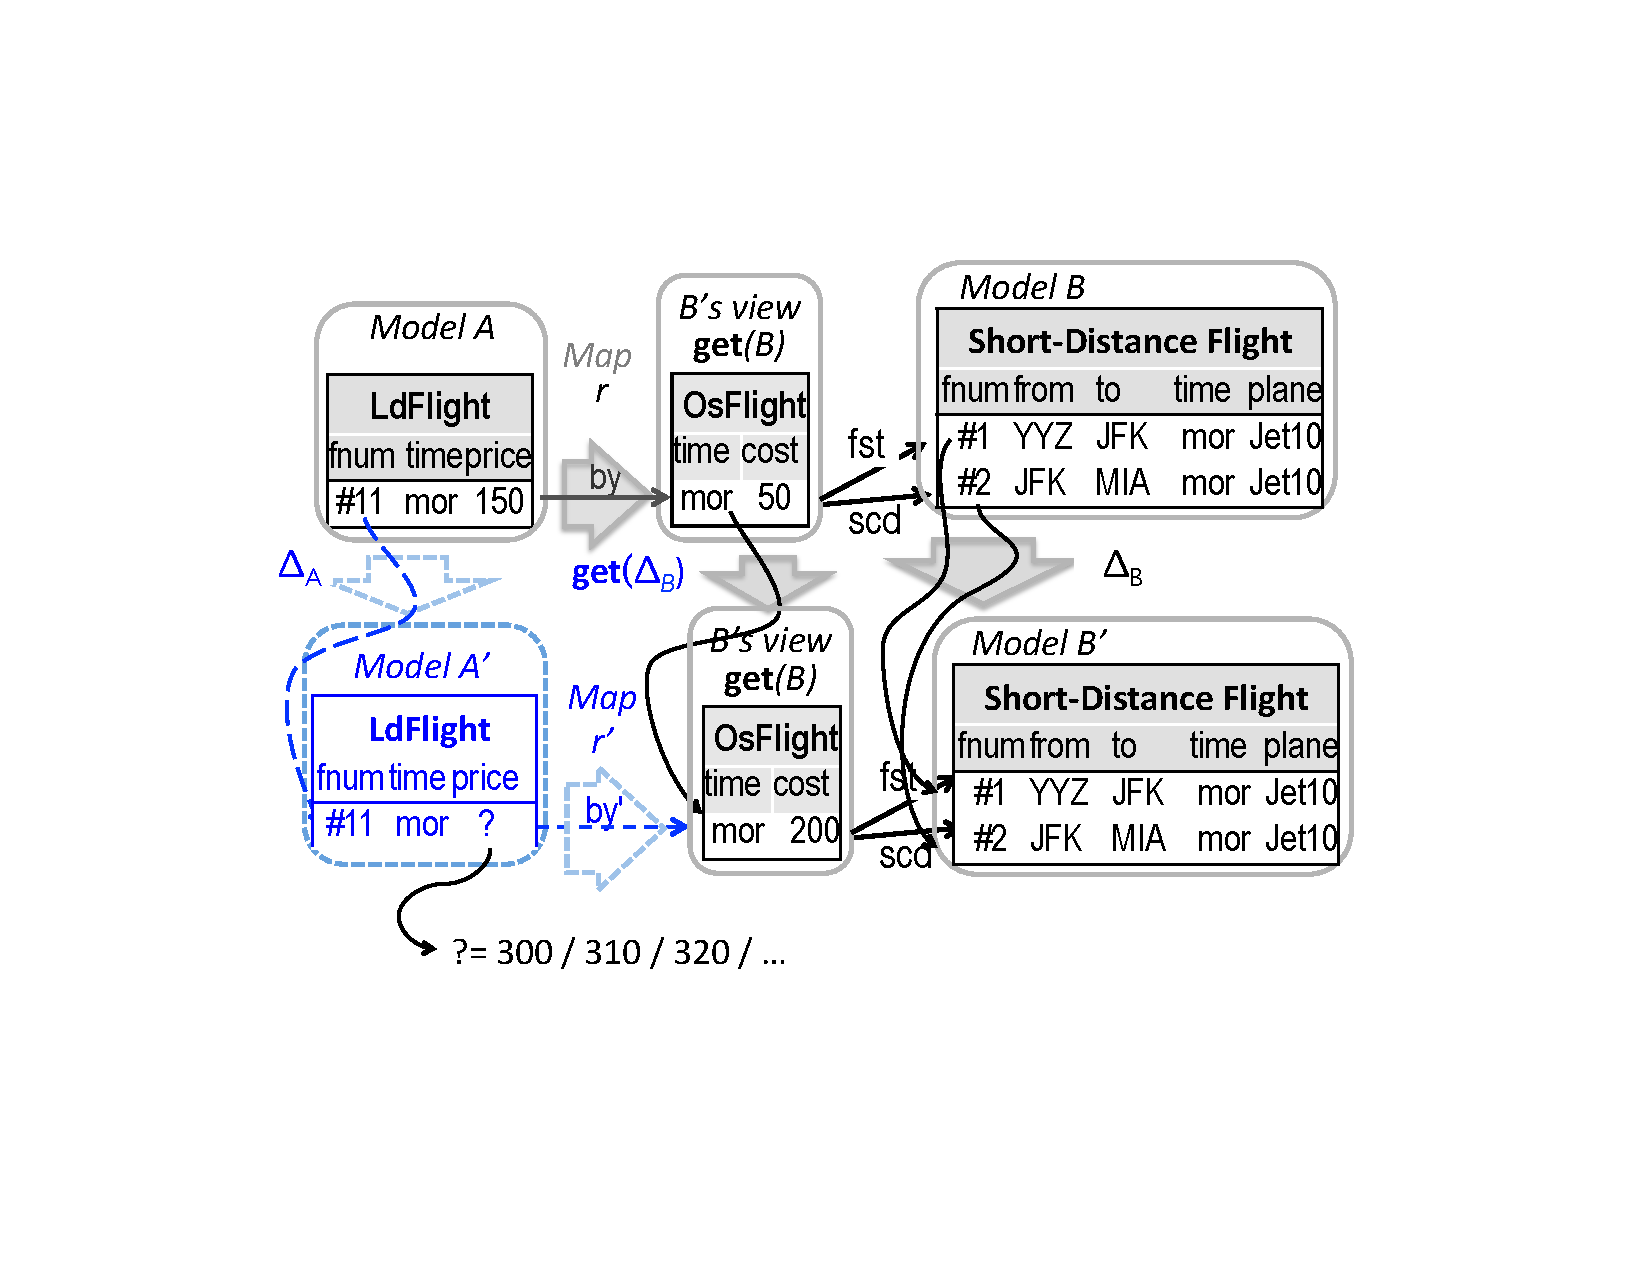
\includegraphics[width=100mm]{images/leastChange}
\caption{What is the Least Change to make Model A and B aligned again}
\label{fig:leastChange}
\end{figure}

Like the previous part this is the general issue that come up in the Incremental synchronization scenarios. This {\em least/minimal} change application on the target model to establish the alignment again between models is getting more complicated when the relationship among them getting complicated and also the models expressed by TAG.  There are some works in the literature which claims doing an incremental synchronization \cite{giese2009:IncrementalSynch}, while without precise definition of the {\em private/shared} parts on the models and also the concept of the {\em minimal/least} change, the claim could not be neither verified nor compared with other approaches.

\subsubsection{Concurrent synchronization and conflict resolution.}
As we already discussed in section \ref{sub:synchSpace}, concurrency dimension seems not to be orthogonal to the org-symm dimension and identifying the role of the concurrency dimension in relationship with all the other dimension would need more study and investigation. 
Yet in the case of concurrent model evolution, there is the concept of conflict resolution which however is not well studied. Suppose that in our example in Section \ref{sub:example}, we have the informational and organizational symmetric scenario. We increase the price of the flight in Model B from 50 to 200 because of the increase in the fuel cost, while at the same time the marketing side decrease the price of the corresponding flight in Model A from 150 to 100 because of the marketing and business decision. At first look this seems to be the distinctive issue of the application domain, but the abstract scenario is a typical situation which arises in synchronization of the info-symmetric/asymmetric and org-semi/full symmetric cases, while simultaneous changes are in conflict. Yet we see we already need to distinguish if these changes belong to the {\em private} part of each models or not. Later we need to decide how to make the alignment procedure with the {\em minimal} change ($\Delta_{B'_1}$ or $\Delta_{B'_2}$ in Figure \ref{fig:conflictResolution}), with the difference that we need to apply the procedure of minimal changes simultaneously to both sides which is a kind of inter-related procedure. 


%:Key leastChange Picture
 \begin{figure}[ht!]
\centering
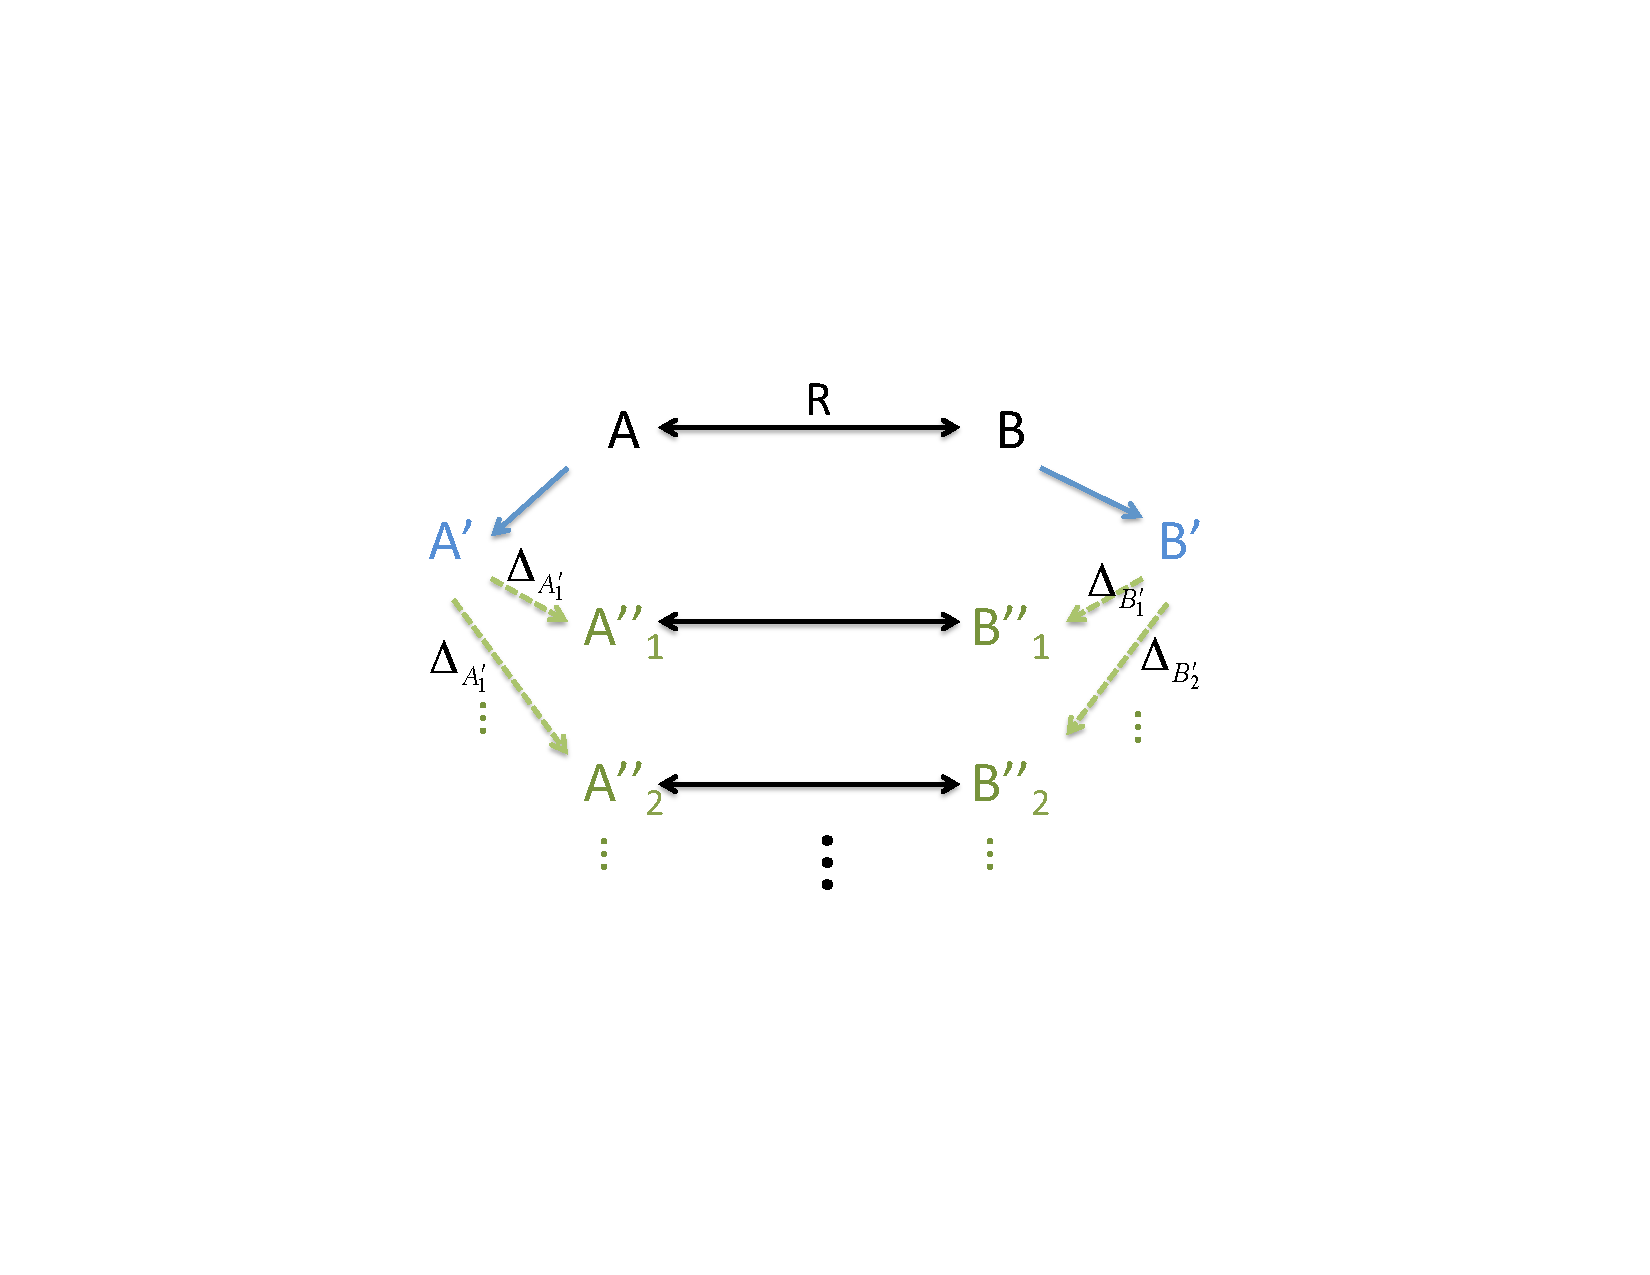
\includegraphics[width=70mm]{images/conflictResolution}
\caption{least change and conflict resolution in concurrent scenario}
\label{fig:conflictResolution}
\end{figure}

The conflict in our example is that the two changes are not compatible (one is increase and one is decrease). The conflict resolution decision is to decide how to resolve this conflict and make the models consistent again. As we already discussed one solution would be giving more priority on one side, say Marketing Model A, calling it {\em master}, and discarding the changes on Model B, then applying the solution of the previous section (least/minimal change on roll backed Model B). But this way the changes and concerns of the technical side in flight example would not be taken into account which might make them upset. The latter approach is not usually a desirable solution in the practical software engineering environment while two teams are working on a set of inter related models while non of them would be happy that their evolutions since their last alignment be disregarded completely. So we need to study and investigate this issue which is termed {\em conflict resolution} in synchronization domain. The desired solution would be the case we change both models to the new state with the {\em least/minimal} changes possible to make both models consistent again. The formulation of this approach is another spot that this thesis is following to address. 


  


%\hl{draw some picture to illustrate the problems}

%\hl{ say that the three identified problems are inter related to each other so need to be resolved in sequence}


%-----------------------
%and  would be the procedure would be to   the price of the flight    
% 
%
% 
%Case one is the case if the synchronization is Orgonizationally asymetric or partial symmetric. 
%
%in {\em batch-update} we don't care 
%
%
%\hl{I think it is possible to move some parts from the background to here like the space of synchronization}
%
%Almost all Synchronization formalization is based on the assumption that we have R clearly defined by some specification constraints \cite { Zinovy Work, TGG (Check it), Xiong work }. But in real application usually R is not clearly defined especially in the complex cases of Model Transformation and Synchronization. For example in TGG Approach \cite{Ehrig:2007:IPB:TGGFromalDef, Konigs:2006:TGGFormalDefSetBased}, Relation between source and target is defined implicitly by TGG rules in constructive and operational way \cite{one of TGG papers}, or in ATL \cite{Jouault:2008:ATL}, Viatra2 \cite{Balogh:2006:Viatra2} R is defined in one direction as a function. Defining a Relation as a function is useful if the nature of the Relation be one-to-many or info-Asymmetric like the Table-View Relation in database domain \cite{cite one of table view papers here}. Apparently the backward transformation of this case would not be a function and would require an update policy to make it a function \cite { cite a update policy paper here}. There are two points regarding our latter discussion that we need to mention out here: (1) there are many cases of model synchronization that are not info-Asymmetric, so the relation definition can not be specified by a function in neither direction (both forward/backward) (2) even in the case of info-Asymmetry, we need to avoid the naive, inefficient and non-intelligence method of batch update of the target for every change that happens on the source. In both above cases (info-asymmetric and info-symmetric) we need to know two important facts: (1) which change in the source imposes changes on the target according to the defined Transformation Function or Relation. we define {\em Private parts} of the source, the entities that any change to them would not impose a change to the target as apposed to {\em Shared parts} which any changes to them requires a change to the target to satisfy the  constraints and  establish the relationship again.\hl{ As we will show by example latter}, distinction of {\em Private} and {\em Shared parts} is not trivial and straight forward result gained out of Relation or Function definitions. (2) if it is determined that the target should be changed (because of {\em Private part} change in source,) how to preserve the relationship(make the target aligned again with the source) by {\em minimum possible change} on the target. In the general case of the info-symmetry(many-to-many Relation) many possible alignments would be possible, however we are interested in one(or maybe a set) of them which are the most desirable(minimum possible change on the target). \hl{we will discuss this case more by an example later}. For addressing this problem it seems that we might need to define some measurements for the updates and calculate the most desirable updates according to these measurement. Hence we would need to identify suitable measurements according to some factors like usability and practical application of synchronization cases.
%if we can address the previous problem in terms of defining a {\em Private} and {Shared parts} formally for the models based on the synchronization scenario, and also identify some criteria for the {\em desirable updates} on the target, then we can give a formal semantic for the concept of incremental synchronization. Therefore synchronization frameworks can be implemented and verified according to that semantics.
%
%
%\hl{ it seems that choosing these} {\em \hl {desirable}} \hl{ changes can not be mechanized?! And they might be just user choices, but in the case that the alternatives are too much for the user to choose there should be some filters which makes them a well-acceptable set of option in some sense out of which user can select. In latter situation those filter parameters can be defined by Transformer Executer (user).}
%
%The extended case of the incremental synchronization formalization would be the {\em concurrent} cases of synchronization which the changes are allowed simultaneously at the source and target in one step.  \hl{ should explain this more}
%
%\hl{QVT-R {\cite{ QVT-R}} and TGG are two approaches that can be  used for Relation Definition among two models in industry, so try to demonstrate the problem by some example based on these two approaches. (What are the other Relational Languages for Relation definition among two models. )}
%
%
%Steven Criticises on the QVT-R semantics!
%
%
%\hl {following  can be moved to approach part} 
%
%Solution: some speculation
%defining a transformation as a function is ATL and Viatra2 is easier than QVT-R, so maybe better idea to have two functions which is practical than one function and let the tool keep the properties among them in according to the constraint that user desire to be maintained by the tool. I mean give the option to the user to choose that criteria getput, hipocratic, invertability, undoable, and .... in maintained for these two functions in pair (forward/backward). since it makes the transformation writting for users easy and practical.
%----

%\hl{the following part should be commented or moved to the methodology and approach section}
%( one look is that looking a the transformation functions defined in ATL and Viatra, and see how they define that function. according to that function the source is sliced into some pieces which each piece is mapped to one target . Reverse looking at this function is a kind of defining half of the full relation in a way that $t \in T $ there exist many $ s \in S$ where $s R t$ .  so out of forward transformation function (lets take it as total just by mapping non-mappable cases (not transferable cases) to null) we can get the half of the relation like $\{s_1 R t_1, s_2 R t_1,  s_3 R t_1, s_4 R t_2 , s_5 R t_3 , ...\}$, we can look at that like $\{\{s_1, s_2,  s_3\} R t_1,\{s_4, s_5\} R t_3\}$ too. Forward transformation function is not always surjective. By the reverse case (backward function) we would have the other half of R $\{ t_1 R s_1, t_2 R s_1,  t_3 R s_1,t_4 R s_2 , t_5 R s_2 ...\}$, we can look at that like $\{\{t_1, t_2,  t_3\} R s_1, \{t_4, t_5\} R s_2 ...\}$ or reverse of it $\{s_1 R \{t_1, t_2,  t_3\} , s_2 R \{t_4, t_5\} ...\}$. so the question is that if these two functions together define the desired Relation R?! I think this is closely related to the constraints that forward and backward transformation should preserve some constraints like hipocraticness(check and force), inevitability, GetPut and ....) to be a BX. They should be studied more!!!!
%Another thing that come to my mind is that it can be related to meta-models too! so meta-models for sure are involved in definition of this private and shared parts.





%\subsection{Example Demonstrating the Problem}
%\hl{I should add example to demonstrate the problem with some examples.}
% Here we are going to show two examples demonstrating the issues related to the {\em Private} and {\em Shared} Parts. Look at the Figure \ref{fig:Example1Pic}. {\em People} Table(Model Space A) representing the records(Models) of People while {\em Employee} Table(Model Space B) representing Employee records. The Relation $R$ between {\em People} and {\em Employee} is that each person is related to the employee with same \verb+Name+ and the \verb+age+ : 
% 
% \hl{(one tricky thing is that how to represent the example 1 Model spaces with TAG)}
% 
%$ \forall a\in A$ and $\forall b \in B,  (a,b) \in R$ if $a.Name=b.Name$ and $a.Age=b.Age$
%
%According to above relation \verb+John+ and \verb+Mike+ record are related to each other.  In first look it seems that the \verb Name and \verb Age are the {\em Shared} part of {\em People} and {\em Employee} in the sense that their changes in each table will cause a change in another table. This result is also can be seen by looking at the Relation Definition above. We can say since the names of the elements(\verb+Name+ and \verb+Age+) are literally exists in the Relation Definition, so those elements are part of the {\em Shared} entities. But when we change the \verb+Bdate+ content in the {\em People}, it would also cause a change in the Employee \verb+Age+ in Employee table. So Bdate Changes should also propogate to the Employee too. That is because of internal functional dependancy \cite{Databasebook} between the Age and Bdate in People table.

%Models in general sense are not as simple as records. as we showed in Section \ref{TAG} they can be formally represented by Typed Attributed Graph. The Notion of the dependancy between the data items in the record can be generalized to the cross cutting constraints between the model elements inside the Graph. So in that sens it is not trivial to distinguish the {\em Private} and {\em Shared parts} out of looking at the Relation Definition between two Models. \hl{maybe refer to another example with graphs in the following sections}.  In practice, it is also not the case that we always have a clear Relation Defintion literally between two Model spaces in terms of their elements. That is because specifying Relational dependancy between large Model is so complicated as apposed to specifying the Transformers by functions, so latter is preferred -- That is one of the reason why languages like ATL and Viatra2 gained more interest over the relational counterparts like QVT-R and TGG in industry. To this end, further investigation of specification of the {\em Private} and {\em Shared Parts} even specifically in each approach of Model Transformation and Synchronization is necessary. It is worth recalling that the this concept is demonstrating its importance while the changes on one model are so small in comparison to the whole model and we want to make the least effort in maintaining the consistency after these changes. \cite {Gies paper in incremental Graph}

%Another aspect of the problem is identifying the least possible changes in the target for maintaining the consistency relation. Suppose in above example we change the Age Group in Employee table from 1 to 2. The most reasonable option for aleviating the Age and Bdate value in People Table is that reounding them to the nearest lowest and largest value to maintain the Relationship. We call this the {\em Minimum/Least Change} concept. This change is not always in terms of the values as it is in the database tables, and it needs to be defined in terms of Graph structures as of Model representatives. So this needs to be more investigated and studied in terms of Models and Model Incremental Synchronization. It is clear that probably we'd better not to limit the options of changes to exactly one cases (i.e. change Age to 60), but provide the user with a range of most probable options (i.e. 60- 70) rather than (60 - ...).

 


%%:Key Example 1 Picture
% \begin{figure}[ht!]
%\centering
%\includegraphics[width=150mm]{images/example1}
%\caption{People and Employee model spaces}
%\label{fig:Example1Pic}
%\end{figure}


%As another example we are considering the transformation between the rail projects and the petrinet discussed in \cite{Kindler2007:TGGConcepts} using Tripple Graph Grammars \cite{sddsd}


%\hl{ you can take it in a unidirectional domain and study that in that area, I think there should be some text in the literature which covers this topic. for example you wrote a transfo. on ATL from A to B, then A changes, so how to propagate its change to B, not touching unrelated data. That arise the fact that how to extract unrelated data from just unidirectional transformation. In another world How we can get  the relation R from just unidirectional case, in the sense that we almost consider Transfo as a function, so it means that the R is a function. This is not realistic!! in practice , we define Transfo, as a function, but taking the shared part of the target as domain. in that sense yes that is function. but that doesn't mean that whole design space of the Target make that transfo a function. let say an example: we define transfo from class diagram to code : this is function, Does the relation from class diagram to code is function? No,  Why?  because for one class diagram there are many implementations which differ in body of the class methods. so the relation from model to code in not a function. In practice we usually specify this relation as function.  So we can just examine the matter of model synchronization in unidirectionally cases as a special case of bidirectional case. this gives the opportunity to study this area independent of the BX which its result can be later extended to BX.}


\section{Literature Review} 
\label{sec:Lit}

% look at the background def. from draft file and fill out here!

%\hl{you need to mention AGG tool {\cite{Taentzer:AGG:2000zr}} in your proposal! , also SDM {\cite{Fischer:SDM:2000ys}}, also EMF {\cite{Steinberg:EMFBook:2008qf}}}


Talking about model synchronization, we already tied with all other aspects of MDE concepts including : {\em Model Transformation}, {\em Meta-Modeling}, {\em Model Specification Language}, {\em Constraint} and {\em Bidirectional Model Transformations(BX)}. At the moment there are many research activities progressing in each area independently and inter-relatively. 

% Talk about BX
% you can cite crystoph fwork on bidirectional transfo *(japan paper), steven on lanscape of bx
%Cite QVT and semantic issues
%Cite lense word
%Cite boomerang and ground tran
%Cite zinovy paper on algebraic approach on Synch and also Delta lenses
Looking at {\em models} as {\em Graphs}, {\em Graph Transformation} techniques are considered as a {\em Model Transformation} foundation in that sense. The book in \cite{book:Rozenberg1997} discusses graph grammar and DPO(Double Push out) and SPO(Single Push out) approaches as two well-known specification for {\em rule application} definition in graph transformation . Another book \cite{book:Ehrig2010} discusses some algebraic foundations of graph transformation using Category theory \cite{Barr:CATBook:1999dz, Awodey:CATBook:2009fv}. These two books are providing informative materials in domain of graph grammars and graph transformation which are closely related to model specification and model transformation basics respectively. Attributed Typed Graph(ATG) are introduced in \cite{Ehrig:2006:OverviewOfFormalConcept} as a formal representation of Models. %There are some alternatives for ATG specification which are also discussed in \cite{ other approach of Attributed typed graph}. 
The Attributed Graph Grammar System(AGG) is a tool which provides some feature for implementation of the ATG \cite{AGG:Website,Taentzer:AGG:2000zr}. Ecore is an implementation of the OMG meta-modeling standard which exist inside Eclipse Modelling Framework (EMF) \cite{Steinberg:EMFBook:2008qf} and many implemented tools are using it to specify meta-modeles in their environment specification. KM3 \cite{KM3:2006ve} is another meta-modeling specification language which is closer to objecte oriented style of class definition.


There are many research at the moment progressing on {\em Graph Transformation} and also some academic tools have been implemented for them. \cite {atom3:Lara:2002qf,AGG:Website, fujaba:website, anjorin2011:emoflon}. Among them {\em Triple Graph Grammars}(TGG) as an extension of regular graph grammars and their tools holds more than 15 year research background \cite{Schurr:2008:15Years} and some successful application. %\cite{ you can cite some TGG application here!!}. 
TGG rules are specifying source and target model evolution in a constructive manner. It is introduced by Andy Sh\"{u}re  in \cite{Schurr:1995:TGGIntro} and formally defined in \cite{Konigs:2006:TGGFormalDefSetBased}, \cite{Ehrig:2007:IPB:TGGFromalDef} and \cite{Golas:2012:TBG:TGGRecentFormalDef} recently. TGG approach is taking graph grammars as a triple of {\em source}, {\em correspondence}, and {\em target} models and defining the relationship between them as a Triple Graph Grammar Rules \cite {Kindler2007:TGGConcepts}. TGG is considered as a Graphical Bidirectional Transformation Languages (BX) too, which forward and backward rules can be extracted from the {\em Triple Rules} in a straight forward manner\cite {Kindler2007:TGGConcepts}. Some properties of 
 of TGG like {\em Functional Behaviour}, {\em Correctness}, {\em Completeness}, and {\em Termination} are formally studied here \cite {Hermann:2010:FAF:FunctionalBeh, Ehrig:2009:OCC:OnTheFly, Ehrig:2008:RMT:OnTheRel,Golas:2012:TBG:TGGRecentFormalDef}. Inheritance, concurrency and application condition in TGG approach are discussed here \cite{TGG:Inheritance:Golas:2012ys, hermann2012:concurrent, TGGAppCondition:Golas:2011zr}
 
 
 % talk about TGG Tools
Besides the Theory of the TGG there are some tools developed for that in academia and some of them applied successfully for industrial projects \cite{Giese:autosar:2009cr}. Among these we can mention MoTE \cite{giese2012:Bridging}, eMofelon \cite{anjorin2011:emoflon}, TGG Interpreter \cite{greenyer2008:TGGInter} and Emorf \cite{klassen2012:emorf}. Although Bi-directionality of the TGG provides some advantages over its usage in term of providing the consistent forward and backward rules for granted, at the same time its usage is limited in defining complex transformation scenarios which are demanded in most industrial cases \cite{Patzina:ATLvsSDM:2012oq}. Besides there are still some space left for research to formalize the application of {\em Constraints} in rule definition which is necessary to use in most of its applications. %\cite{ try to cite something related to constraint on TGG here}.
Giese and Wagner discuss incremental model synchronization implementation in TGG in \cite {giese2009:IncrementalSynch}; But no formal foundation is provided to verify how far their incremental implementation is correct in the sense of being {\em Incremental}. % This is actually one of the objectives of this PhD research to establish a mathematical specification which incrementality of the synchronization can be verifiable. % \hl{Regarding Synchronization Techniques in TGG, {\cite{hermann2012:concurrent}} studies Conflict Resolution strategies in TGG approach. (Maybe you need to read that paper and put some comments here).}

Apart from TGG tools there are some other tools like MediniQVT \cite{ikv-technologies:mediniQVT} %smartQVT \cite{smartQVT} 
based on OMG  QVT specification \cite{OMG:QVT:2011}. Stevens criticise QVT semantics here \cite{steven:QVT-Semantic2010} which is a hinder in QVT proper implementation. Story Diagrams is another approach in combining graph grammars and the Activity diagrams of the UML, for realization of the class operations \cite{Fischer:SDM:2000ys}.

% cite some other transformation languages.
Lenses Framework is discussed in \cite{Hofmann:2011:SymLens}. It is trying to provide a consistent forward and backward transformation out of single specification language. Boomerang framework \cite {Bohannon:2008:Boomerang} is implemented based on that idea. But the language application is limited to String data at the moment and covers info-Asymmetric cases in Synchronization Scenario. There is no discussion on the incremental update integration to the framework and the emphasize in on defining BX language. 
GroundTram \cite {hidaka2011:Groundtram} is another thrend trying to define BX programming languages based on edge-labeled Graphs. They are using $UnQL^+$ language(an Extension of UnQL \cite{buneman2000:UnQL} ) for defining Bidirectional Transformation, but again the emphasize is on the Bidirectionality rather than the incrementality.

%(Should read Zinovy Tile Algebra paper and also Algebraic approach to comment on that)
%(I also need to read xiong paper on incremental approach and comment on that)
%(I also need to read TGG sychronization of Ehrig and Zinovy and comment on that) 

% cite crystoph work on Synch  
%Shynchronization scenarios is categorized in eighteen different categories in \cite{antkiewicz2008:DesigndSpace} 

%Cite Xiong work on Synchronization





%Does it necessary to study synchronization and cuncurrent synchronization in BX domain? It seems no!
%you can take it in a unidirectional domain and study that in that ares, I think there should be some text on th e lirature which covers this topic. for example you wrote a transfo. on ATL from A to B, then A changes, so how to propogate tis change to B, not touching unrelated data. That arise the fact that how to extract unrelated data from just unidirectional transformation. In another world How we can get  the relation R from just undirectional case, in the sense that we almost consider Transfo as a function, so it means that the R is a function. This is not realistic!! in practice , we define Transfo, as a function, but taking the shared part of the target as domain. in that sens yes that is function. but that dosn't mean that whole design space of the Target make that transfo a function. let say an example: we define transfo from class diagram to code : this is function, Does the relation from class diagram to code is function? No,  Why? --> because for one class diagram there are many implementations which differ in body of the class methods. so the relation from model to code in not a function. In practice we usually specify this relation as function.  So we can just examine the matter of model synchronization in unidirectional cases as a special case of bidirectional case. this gives the opportunity to study this area independent of the BX which its result can be later extended to BX.

%-----------------
%Ehrig et al. discusses the fundamentals of algebraic Graph Transformation is a series of books \cite{book:Ehrig2010, book:Rozenberg1997} , and papers \cite{Ehrig:2004:ATGFundemental, Golas:2012:TBG:TGGRecentFormalDef, TGG:Inheritance:Golas:2012ys, hermann2012:concurrent, TGGAppCondition:Golas:2011zr},  defining Attributed Typed Graph as Model, Graph Grammars, TGG formalization, Concurrency in TGG, Application Conditions in TGG and etc. and loot[Some Ref here to TGG, all ref to TGG, GroundTram, , Constraints: donloaded constraint papers, BX: Crystoph paper] . Among aforementioned Subjects the first one, Model Transformation and BX is closely coupled with Model Synchronization. At the moment there are couple of approaches [TGG, Lenses, GroundTram] , languages [Boomrang, ATL, QVT, Viatra2, and many academic tools [AGG, Emofelon, MoTE, TGG-Interpreter, Emorf, MediniQVT]  developed based on those thories and there is active research groups working on them.

%\hl{Mention what is done related specifically to the private/shared parts --> mention gies paper and conflict resolution, no work on least change!!! }

%\hl{ mention the tools related to TGG, TGG-interpreter, Mofelon, Gies tool, emorf, emf, japan tool, mediniQVT, smartQVT, SDM,}




\section{Conclusion and Future work}\label{sec:conclusion}

conclusion goes here...


%\begin{itemize}
%	\item What is this paper is about?!
%	\item What is the problem identified  
%	\item How you gonna approach it.
%	\item if you solve this what will happen (what is the contribution)
%\end{itemize}

Model are formalized as Typed attributed Graph(ref. section \ref{sub:TAG} ), and Deltas (Updates) among them can be considered as morphism between the graphs.  So the models and the morphism are making a category of the TAGraph \cite{book:Ehrig2010}. Further study of the connection between category theory and the Model synchronization with specific focus on the aforementioned problems in section \ref{sec:Problem} could shed more lights these issues and would help to better understanding and formalizing the problems discussed there.  

Beside that looking at different example of model transformation in large scales in practice and investigating them, while keeping in mind the space of the synchronization scenario and also probing the problems and their probable domain specific solution to those problems would help in generalizing the solution to other domain. This is important because at the moment there are different approaches and languages used for model synchronization and transformation(ref.  section \ref{sec:Lit}) and this also happens in different domain of applications \cite{Stevens:Landscape:2008kl, antkiewicz2008:DesigndSpace}. 

So our next steps are divided into two main branches of theoretical investigation of the Category theory and model formalization and the practical and industrial investigation of the synchronization scenarios with the focus of the identified aforementioned problems, where we tend to join these two path together, However we are not taking them separate from the beginning. 

We expect that the resolution of the issues in this thesis proposal will contribute to making the synchronization procedure and application more efficient and practical which will be an advancement in providing a technical and theoretical support in Domain of MDE in its specific and also in its broader sense \cite{Czarnecki:BX:2009tg}






\pagebreak

% This includes all references from the BibTeX file in the bibliography
\nocite{*}

\begin{spacing}{1}
  \bibliographystyle{plain}
  \bibliography{ref-list}
\end{spacing}

%-----------This is commented Appendix Part---------------
%\appendix
%\section{Further Open Problems}
%\label{appendix:OpenProb}

\end{document}
